% Copyright 2009 by Tomasz Mazur
%
% This file may be distributed and/or modified in all ways.


\documentclass[xcolor=pdftex,t,11pt]{beamer}

%%%%%%%%%%%%%%%%%%%%%%%%%%%%%%%%%%
%       SET OPTIONS BELOW        %
%%%%%%%%%%%%%%%%%%%%%%%%%%%%%%%%%%

\usepackage{xspace}
\usepackage{subfig}
\usepackage{adjustbox}
\usepackage{pifont}
%\usepackage{mdframed,framed}
 \usepackage{adjustbox}
\usepackage{xcolor,colortbl}
 \newcommand{\hpathlen}{\ensuremath{\mathit{pathLength}}\xspace}
\newcommand{\halloc}{\ensuremath{\mathit{new}}\xspace}
\newcommand{\hassign}{\ensuremath{\mathit{assign}}\xspace}
\newcommand{\hlookup}{\ensuremath{\mathit{lookup}}\xspace}
\newcommand{\hupdate}{\ensuremath{\mathit{update}}\xspace}
\newcommand{\halias}{\ensuremath{\mathit{alias}}\xspace}
\newcommand{\hisnull}{\ensuremath{\mathit{isNull}}\xspace}
\newcommand{\hispath}{\ensuremath{\mathit{isPath}}\xspace}
\newcommand{\hcircular}{\ensuremath{\mathit{circular}}\xspace}
\newcommand{\id}{\ensuremath{\mathrm{id}}\xspace}
\newcommand{\hsubdivide}{\ensuremath{\mathit{subdivide}}\xspace}
\newcommand{\hfresh}{\ensuremath{\mathit{fresh}()}\xspace}
\newcommand{\shakira}{{\sc Shakira}\xspace}
\newcommand{\hnull}{{\bf null}}
\newcommand{\xmark}{\ding{55}}

\usetheme[
% Toggle showing page counter
pagecounter=true,
%
% String to be used between the current page and the
% total page count, e.g. of, /, from, etc.
pageofpages=of,
%
% Defines the shape of bullet points. Available options: circle, square
bullet=circle,
%
% Show a line below the frame title. 
titleline=true,
%
% Set the style of the title page (true for fancy, false for standard)
alternativetitlepage=true,
%
% Institution logo for fancy title page.
% Comment out to remove the logo from the title page.
% IMPORTANT: THERE IS A BUG IN SOME VERSIONS OF PDFLATEX AND FONTS
% ON THE LOGOS ARE NOT RENDERED PROPERLY. IN SUCH A CASE ADD `2` 
% TO THE NAME OF THE LOGO, E.G. comlab2 INSTEAD OF comlab
%titlepagelogo=images/titlepage/ou,
%
% Department footer logo for fancy title page
% Comment out to remove the logo from the footer of the title page/
% IMPORTANT: THERE IS A BUG IN SOME VERSIONS OF PDFLATEX AND FONTS
% ON THE LOGOS ARE NOT RENDERED PROPERLY. IN SUCH A CASE ADD `2` 
% TO THE NAME OF THE LOGO, E.G. comlab2 INSTEAD OF comlab
%titlepagefooterlogo=images/titlepage/comlab,
%
% Institution/department logo for ordinary slides
% Comment this line out to remove the logo from all the pages.
% Available logos are: ou, comlab, comlabinline, comlabou
% IMPORTANT: THERE IS A BUG IN SOME VERSIONS OF PDFLATEX AND FONTS
% ON THE LOGOS ARE NOT RENDERED PROPERLY. IN SUCH A CASE ADD `2` 
% TO THE NAME OF THE LOGO, E.G. comlab2 INSTEAD OF comlab
%ordinarypageslogo=TU-Signet,
%
%
% Add watermark in the bottom right corner
%watermark=<filename>,
%
% Set the height of the watermark.
%watermarkheight=100pt,
%
% The watermark image is 4 times bigger than watermarkheight.
%watermarkheightmult=4,
]{Torino}

% Select color theme. Available options are:
% mininmal, greenandblue, blue, red
\usecolortheme{blue}

%Select different font themes.Available options are:
% default, serif, structurebold, structureitalicserif, structuresmallcapsserif
\usefonttheme{structurebold}


\pgfdeclareimage[height=6ex]{ou-logo}{ou}

\logo{\pgfuseimage{ou-logo}}

\usepackage{pgf}

\pgfdeclareimage[height=6ex]{ou-logo}{ou}

\logo{\pgfuseimage{ou-logo}}

\usepackage{listings}

\lstset{language=C,
 basicstyle=\normalsize
 }

\usepackage{ifthen}

\usepackage{pgf}
\usepackage{tikz}
\usetikzlibrary{arrows, automata, shapes.multipart, chains, positioning, fit, graphs, spy, shapes, backgrounds, patterns}

\usepackage{color}
\definecolor{light-gray}{gray}{0.80}
\definecolor{green}{rgb}{0.30588, 0.60392, 0.023529}     % #4e9a06


\newenvironment<>{codeblock}[1][]{%
  \setbeamercolor{block title example}{fg=white,bg=blue!75!black}%
  \begin{block}#2[#1]}{\end{block}}

  \newenvironment<>{examplesecond}[1]{%
  \setbeamercolor{block title}{fg=white,bg=blue!75!black}%
  \begin{block}#2{#1}}{\end{block}}

  

%%%%%%%%%%%%%%%%%%%%%%%%%%%%%%%%%%
%       PRESENTATION INFO        %
%%%%%%%%%%%%%%%%%%%%%%%%%%%%%%%%%%

\title{\fontsize{11}{12}\selectfont Automated Formal Synthesis of Digital Controllers for State-Space Physical Plants}
\subtitle{CAV 2017}
\institute{\normalsize Diffblue Ltd., \\University ~of ~Oxford, \\Federal University of Amazonas}
\date{}
\author{\normalsize Alessandro Abate, Iury Bessa, Dario Cattaruzza,\\
  Lucas Cordeiro, {\bf Cristina David}, Pascal Kesseli,\\
  Daniel Kroening and Elizabeth Polgreen}

\begin{document}


%%%%%%%%%%%%%%%%%%%%%%%%%%%%%%%%%%
%       SLIDE DEFINITIONS        %
%%%%%%%%%%%%%%%%%%%%%%%%%%%%%%%%%%

\begin{frame}[plain]
  \titlepage
  \vspace{-7.5cm}
    
\includegraphics[width=.15\textwidth]{figures/aec-badge-cav.pdf}
\end{frame}


%\section{$\checkmark$ Motivation}

%\section{$\checkmark$ Contributions}
%\subsection{Example}
%\subsection{Cristina Says Something}

\begin{frame}{Motivation}

  %Cyber-physical systems (CPS) are becoming ubiquitous in our daily life.
  % use a better figure for cyber-physical systems
%\vspace{-1cm}

  \begin{center}
\vspace{-.5cm}
    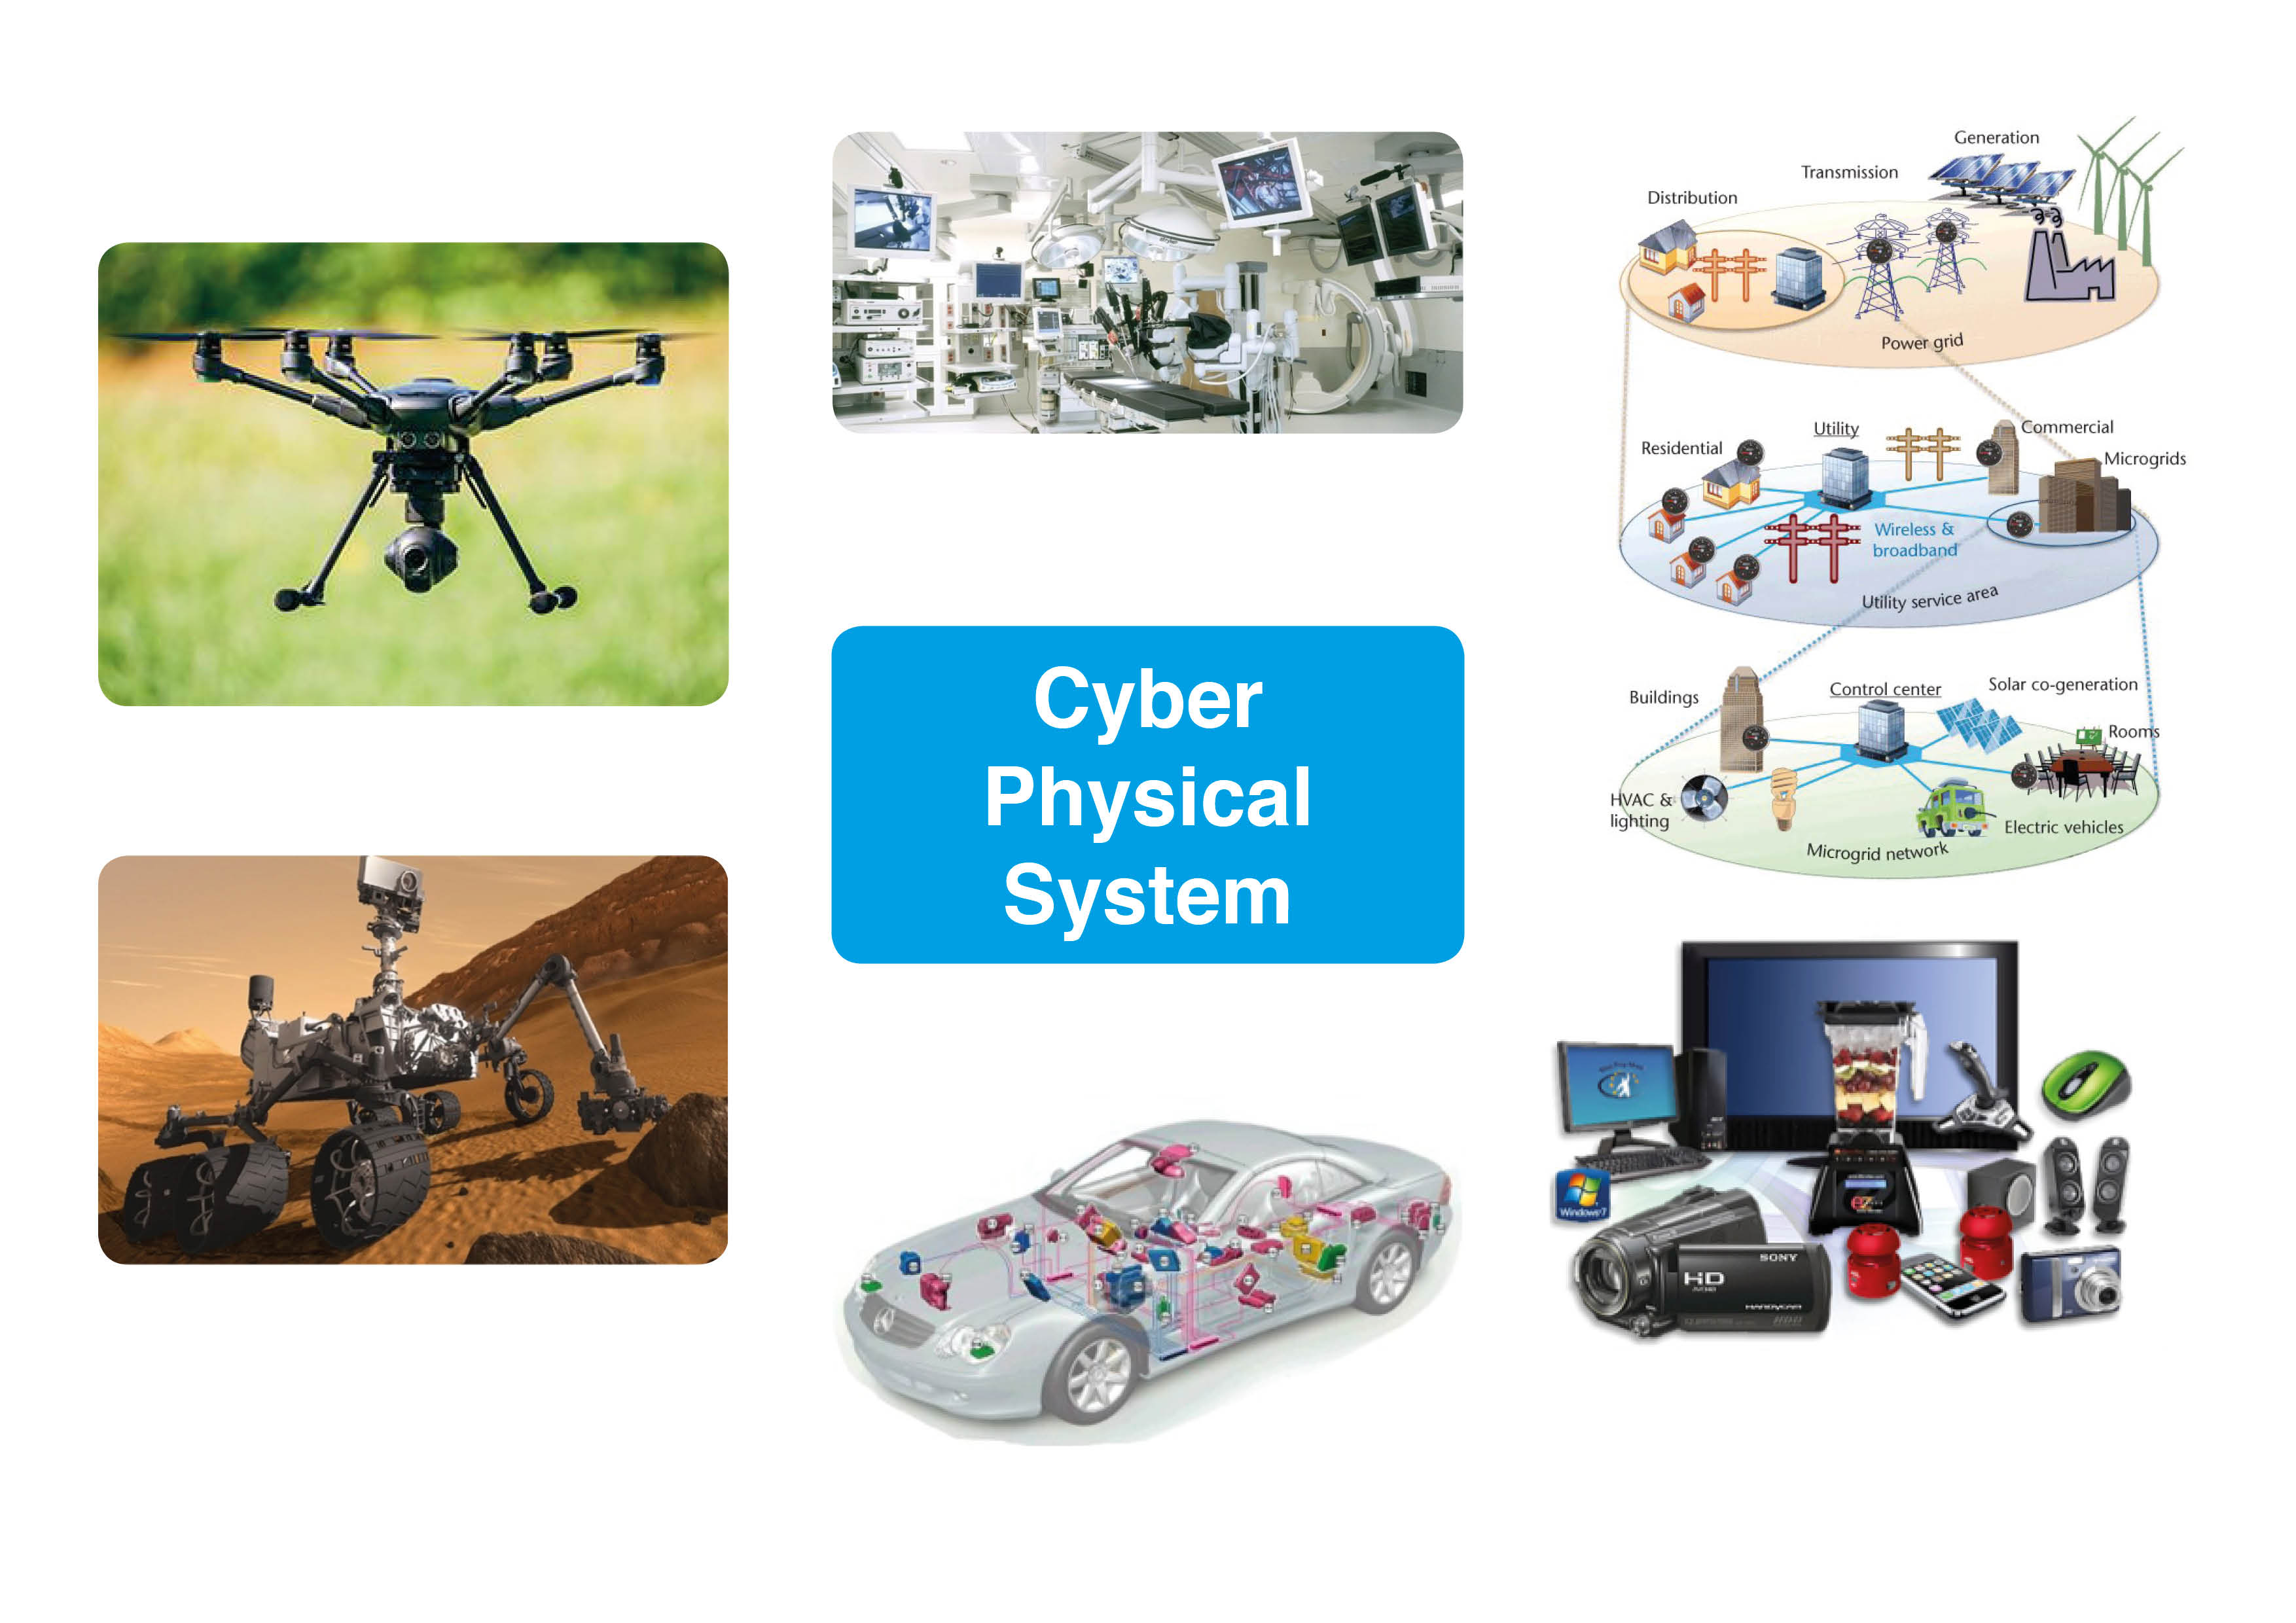
\includegraphics[width=.75\textwidth]{figures/CPS.jpg} 
  %% \begin{tabular}{lll}
  %%   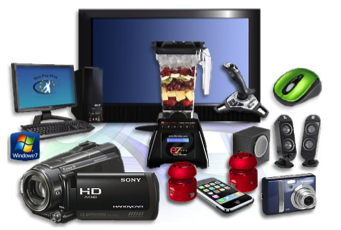
\includegraphics[width=.2\textwidth]{figures/step1_FigureD.png} &
  %%   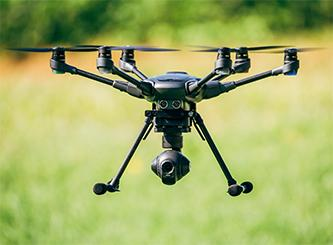
\includegraphics[width=.25\textwidth]{figures/drone.jpg} &
  %%   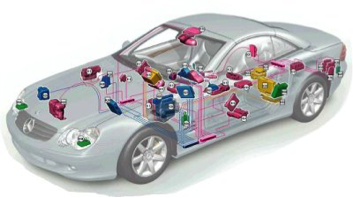
\includegraphics[width=.25\textwidth]{figures/step1_FigureC.png}\\
  %%   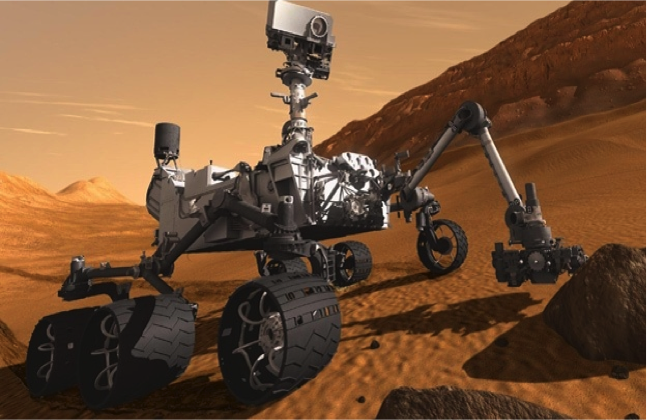
\includegraphics[width=.25\textwidth]{figures/step1_FigureB.png}&
  %%   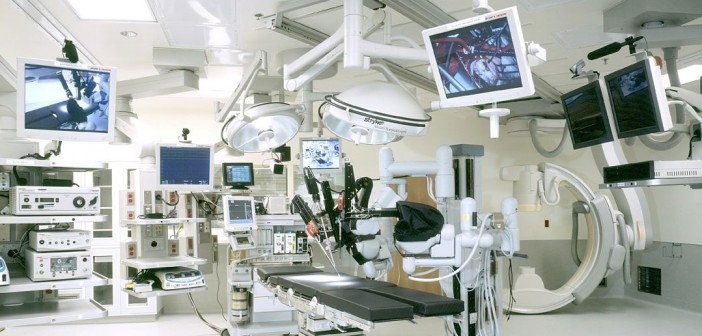
\includegraphics[width=.25\textwidth]{figures/medical.jpg} &
  %%   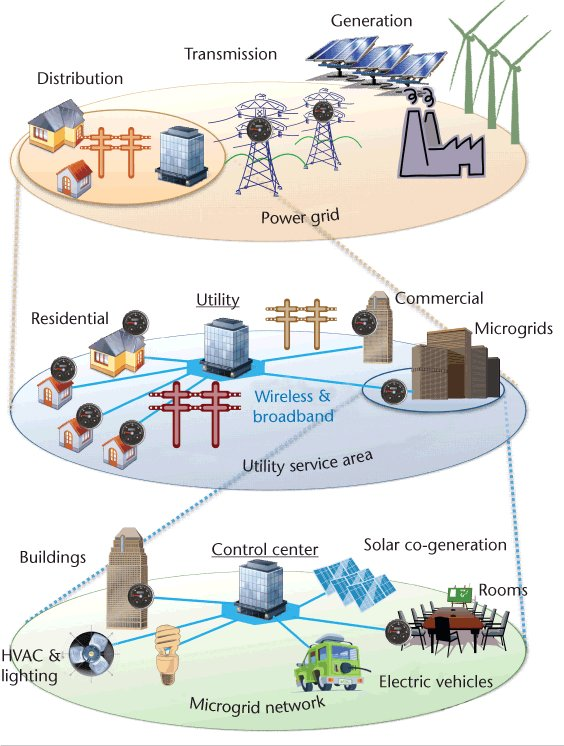
\includegraphics[width=.15\textwidth]{figures/intelligent_building.jpg}    
  %%   \end{tabular}
\end{center}
 

% smart spaces, intelligent transportation, medical equipment, sensors, robotics. 
 
%CPS = {\bf digital controllers} embedded within {\bf physical systems}.
\uncover<2>{
 \vspace{-.5cm}
  \small
{\bf Automatically synthesise feedback digital controllers that ensure {\color {red} stability} and {\color {red} safety}}.}

\end{frame}

%% \begin{frame}{Example}
  
%%   \begin{center}

%%   \begin{tabular}{ll}
%%  \includegraphics[width=.4\textwidth]{figures/aircon.jpg}&
%%  \includegraphics[width=.3\textwidth]{figures/thermostat.jpg}
%%   \end{tabular}

%%   \end{center}

%%   \vspace{.5cm}
  
%%  The thermostat must control the aircon such that the ambient temperature is stable and within
%%  safe bounds.
 
%% \end{frame}

\begin{frame}{Problem specification}
\vspace{-1cm}
  \begin{center}
  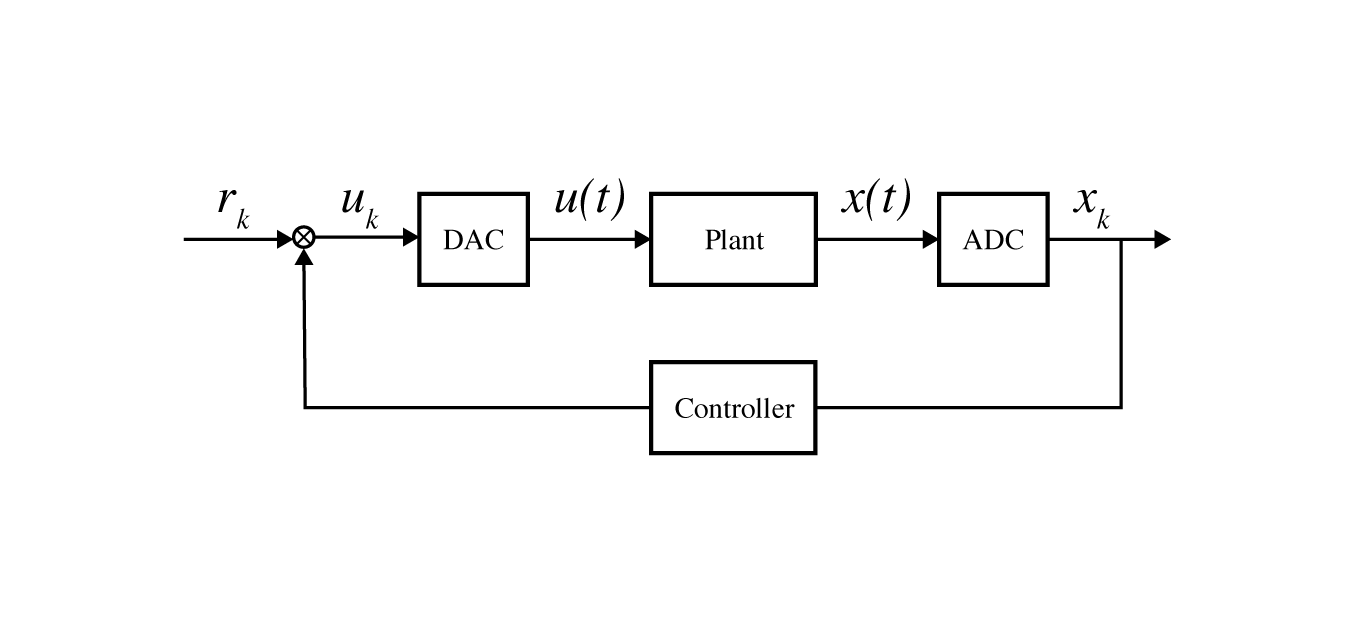
\includegraphics[width=.5\textwidth]{figures/spirals/diagram-14.png}
  \end{center}
  
  %\small
  %% \begin{itemize}
  %% \item {\bf Closed-loop} system.
 
  %% \item {\bf Single Input Single Output (SISO) Linear Time Invariant (LTI)} plant models.

  %% \item {\bf State-space} representation. % of the evolution of the plant
%
  %\begin{align*}
  {\bf Continuous-discrete system}
  \begin{itemize}
\item Plant: $\dot{x}(t) = Ax(t)+ Bu(t), \quad t \in \mathbb R_0^+,~x(0)=initial~state$ 
%\end{align*}
%
\item State-feedback controller:   \only<1>{$u_k = r_{k} - C x_k$}\only<2->{$u_k = - C x_k$}
\end{itemize}

   %[figure] switch to figure with converters.
  %% \only<2>{{\color {red} {\bf Challenge:}} This is a hybrid model, where the plant exhibits {\bf continuous behavior}, whereas the controller operates in {\bf discrete time} and over a {\bf quantized domain}.}

  % This depends on external non-determinism in the form of input signals

  %// We want to to manipulate the properties and behaviors of the plant.

  %% // For this we use a state-feedback controller (the control action from the controller is dependent on the process output)

\end{frame}

\begin{frame}{Our approach}
\vspace{-1cm}
  \begin{center}
    \only<1>{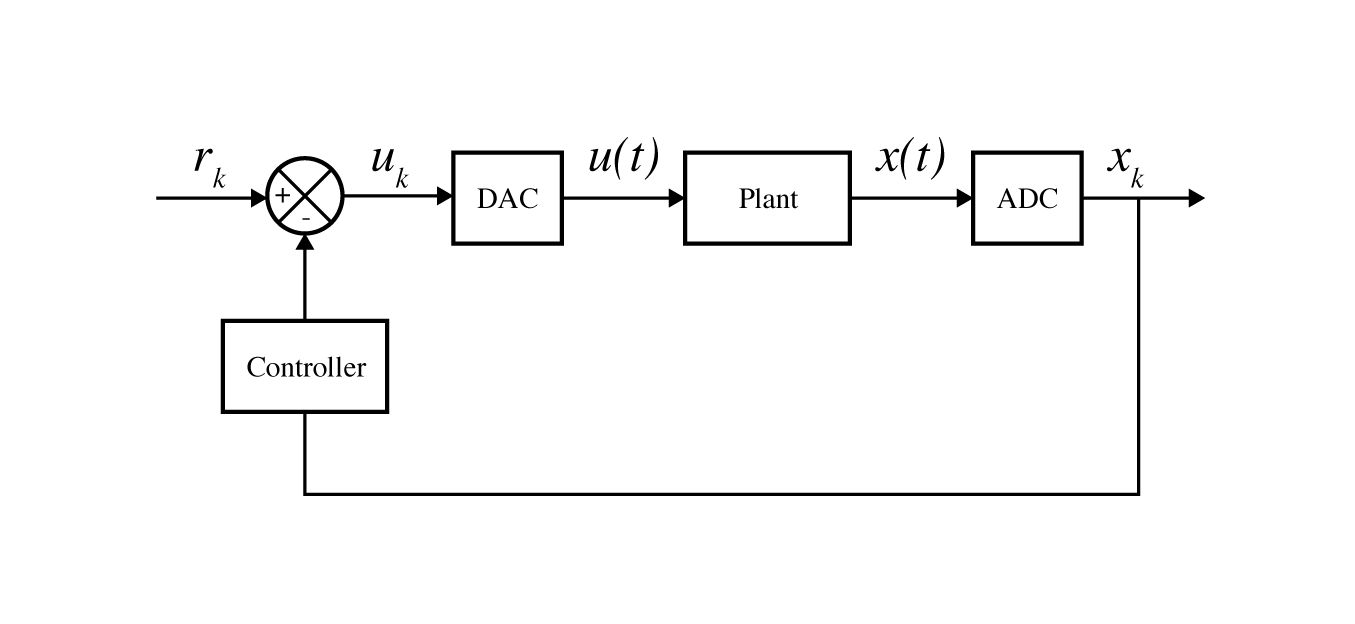
\includegraphics[width=.5\textwidth]{figures/spirals/diagram1.png}}
    \only<2->{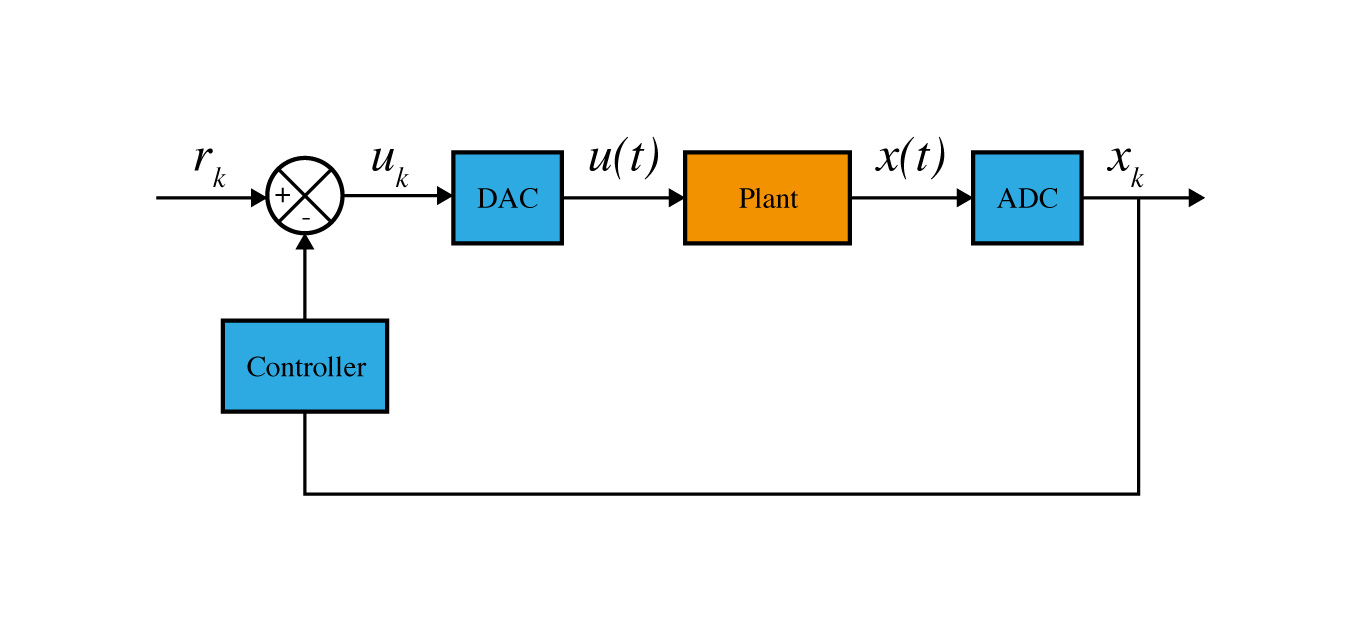
\includegraphics[width=.5\textwidth]{figures/spirals/diagram2.png}}
  \end{center}

\footnotesize

\vspace{-.5cm}
{\bf 1. Translate to a single digital domain}
\begin{itemize}
 \item Plant: $x_{k+1} = A x_k+ B u_k$
 \item State-feedback controller: $u_k = - C x_k$
 \item Finite precision %: $\langle I_p,F_p \rangle$, $\langle I_c,F_c \rangle$, $I_p{\geq}I_c$, $F_p{\geq}F_c$
%\item Controller: manipulates state values at lower precision $\langle I_c,F_c \rangle$
  \end{itemize}
\vspace{.2cm}
 \uncover<2->{{\bf 2. Evaluate sources of numerical error}
  \begin{itemize}
  \item {\color {orange} FWL effects on the plant} (interval arithmetic)
  \item {\color {blue} FWL effects on the controller} (additive noise)
  \end{itemize}
  }
\vspace{.2cm}
  \uncover<3->{{\bf 3. Apply program synthesis}} 

\end{frame}
  
  
  %% The resulting closed-loop system is
  %% a program with a loop that operates on bit-vectors encoded
  %% using fixed-point arithmetic with finite word length (FWL).
  %% The three effects of 1. uncertainties, 2. FWL representation
  %% and 3. quantization errors are incorporated into the model,
  %% and are taken into account during the CEGIS-based synthesis
  %% of the control software for the plant.
  
%% \begin{frame}{Motivation}
%% Linear Time Invariant (LTI) models represent a broad class of dynamical sys-
%% tems with significant impact in numerous application areas such as life sciences,
%% robotics, and engineering [2, 11]. The synthesis of controllers for LTI models
%% is well understood, however the use of digital control architectures adds new
%% challenges due to the effects of finite-precision arithmetic, time discretization,
%% and quantization noise, which is typically introduced by Analogue-to-Digital
%% (ADC) and Digital-to-Analogue (DAC) conversion.
%% \end{frame}

%% \begin{frame}{Closed-loop control system}
%%   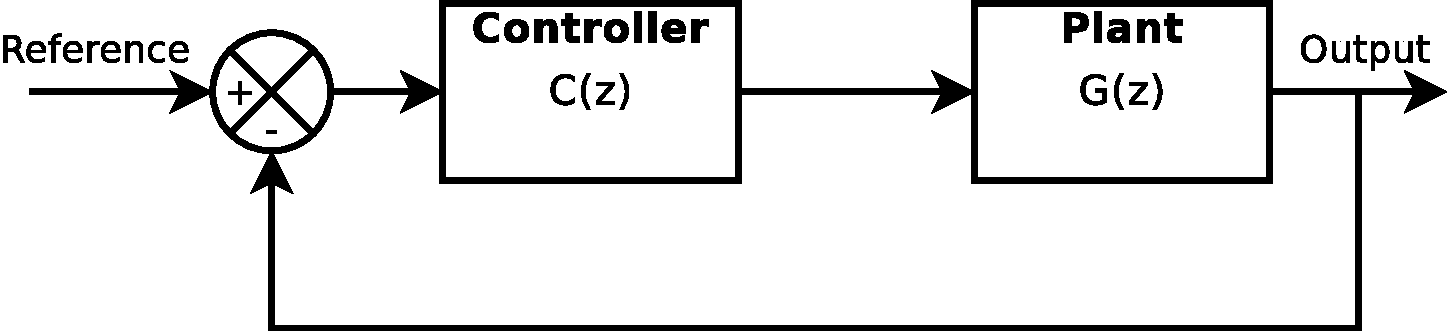
\includegraphics[width=\textwidth]{closedloopseries.pdf}

%%   Outputs of discrete plant G(z) are fed back and compared to a
%%   reference signal to which a controller C(z) should steer.

%%   Representation: state-space LTI model.
%% \end{frame}

%% \begin{frame}{Our approach}

%%   Translate everything into the digital domain.

 
%% \end{frame}

%% \begin{frame}{State-space representation}
%% \begin{itemize}
%% %% \begin{align*}
%% %% \dot{x}(t) = Ax(t)+ B u(t), \quad x \in \mathbb{R}^{n}, u \in \mathbb{R}^m, A \in \mathbb{R}^{n \times n}, B \in \mathbb{R}^{n \times m}, 
%% %% \end{align*}
%% %% %
%% %% where $t \in \mathbb R_0^+$, where $A$ and $B$ are matrices that fully
%% %% specify the continuous plant, and with initial states set as $x(0)$.

%% %% This is soundly discretized in time into:
%% \item  {\bf Discretized plant:} 
%% \begin{align*}
%%  & x_{k+1} = A x_k+ B u_k \qquad k \in \mathbb N, x_k \in \mathbb{R}^{n}, u_k \in \mathbb{R}^m, A \in \mathbb{R}^{n \times n}, B \in \mathbb{R}^{n \times m}\\
%% & u_k = r_{k} - K x_k \\ 
%%  & x_0=initial~state 
%% \end{align*}
%% %% where $k \in \mathbb N$ and $x_{0}$ is the initial state,
%% %% $A_d$ and $B_d$ denote the matrices that describe the discretized plant dynamics.

%% \item {\bf Fixed-point representation:}
  
%%   Plant: $\langle I_p,F_p \rangle$

%%   Controller: $\langle I_c,F_c \rangle$

%% %% \begin{flalign*}
%% %% &x_{k+1} =\mathcal{F}_{\langle I_p,F_p \rangle}(A) \mathcal{F}_{\langle I_p,F_p \rangle}(x_{k}) + \mathcal{F}_{\langle I_p,F_p \rangle}(B)\mathcal{F}_{\langle I_p,F_p \rangle}(u_{k}) \qquad \qquad \quad\\
%% %% &u_{k}=-(\mathcal{F}_{\langle I_c,F_c \rangle}(K)\cdot\mathcal{F}_{\langle I_c,F_c \rangle}(x_{k}))
%% %% \end{flalign*}

%% \end{itemize}

%We synthesize for requirements over this discrete-time domain.

%% The behavior of a system is represented via a state
%% evolution equation $x(n+1)$ and an instantaneous output equation $y(n)$, as
%% follows:
%% %
%% \begin{equation}
%% \begin{split}
%% x(n+1) &= A x(n) + B u(n)
%% \\
%% y(n) &= C x(n) + D u(n), 
%% \end{split}\label{eq:ss-example}
%% \end{equation}
%% %
%% where $A$, $B$, $C$ and $D$ are matrices that fully specify the model. 
  
%\end{frame}

%% \begin{frame}{State feedback architecture}
%% %The most basic feedback architecture is the state feedback one, 
%%   %where
%%   The control action $u_k$ is computed by: 
%% %
%% \begin{equation*}
%% u_k = r_{k} - K x_k
%% \end{equation*}
%% %
%% Here, $K \in \mathbb{R}^{m \times n}$ is a state-feedback gain matrix, 
%% and $r_{k}$ is a reference signal (again digital).   
%% %
%% The closed-loop model then takes the form 
%% \begin{align*}
%% x_{k+1} = ( A_d - B_d K ) x_k + B_d r_k
%% \end{align*}

%% \end{frame}  

%% \begin{frame}{Objectives}
%% The gain matrix $K$ can be set so that the closed-loop discrete dynamics are
%% shaped as desired: according to a specific stability goal or
%% a quantitative safety requirement.

%% \end{frame}  

%% \begin{frame}{Novelty}

%% - Quantitative safety requirements are not typical in the digital
%% control literature.
  
%% - We embrace the digital nature of the controller, which
%% manipulates quantized signals as discrete quantities represented with
%% finite precision.
%% \end{frame}  

%% \begin{frame}{Stability of closed-loop systems}

%% Asymptotic stability is a property that amounts to convergence of the
%% model executions to an equilibrium point, starting from any states in
%% a neighborhood of the point.

%% 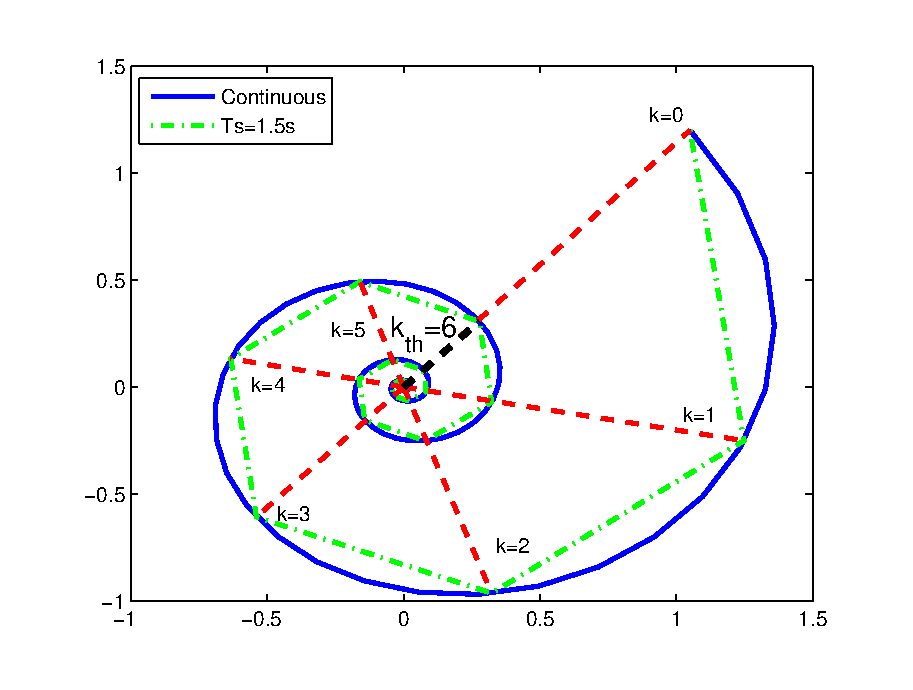
\includegraphics[width=0.4\textwidth]{ct.eps}

%% %% A discrete-time LTI system is asymptotically
%% %% stable if all the roots of its characteristic polynomial (i.e., the
%% %% eigenvalues of the closed-loop matrix $A_d - B_d K$) are inside the unity
%% %% circle of the complex plane, i.e., their absolute values are strictly less than
%% %% one (this simple sufficient condition can be generalised, 
%% %% however this is not necessary in our work).  
%% We express this stability specification $\phi_\mathit{stability}$ in terms of a check known as
%% \emph{Jury's criterion}.
%% %% this is an easy algebraic formula to
%% %% select the entries of matrix $K$ so that the closed-loop dynamics are shaped
%% %% as desired.

%% \end{frame}  

%% \begin{frame}{Safety of closed-loop systems}
%% A safety specification gives raise to a requirement on the states of
%% the model, such that the feedback controller (namely the choice of the
%% gains matrix~$K$) must ensure that the state never violates the
%% requirement.


%% \begin{equation*}
%% \phi_\mathit{safety}\iff \forall k\ge 0.\, \bigwedge_{i=1}^{n}{\underline{x_{i}} \leq x_{i,k} \leq \overline{x_{i}}}
%% \end{equation*}

%% where $\underline{x_{i}}$ and $\overline{x_{i}}$ are lower and upper bounds
%% for the $i$-th coordinate $x_{i}$ of state $x\in \mathbb R^n$ at the $k$-th
%% instant, respectively.


%% This means that the states will always be within an $n$-dimensional hyper-box.


%% \end{frame}

%% \begin{frame}{Sources of uncertainty}

%%   \begin{itemize}
%%     \item (Representation) Numerical error introduced by the
%%       fixed-point numbers employed to model the plant, i.e., to
%%       represent the plant dynamics $A_d$, $B_d$ and $x_k$. We address this
%%       by using interval arithmetic in the verification phase.
%%     \item Quantization error introduced by the digital controller,
%%       which performs operations on fixed-point numbers. We represent this as
%%       nondeterministic addtive noise.
%%   \end{itemize}  

%% %% The physical plant operates in the
%% %% reals, which means our verification phase must also account for the numerical error and quantization errors caused by representing the physical plant at the finite precision $\mathcal{F}_{\langle I_p,F_p \rangle}$.

%% \end{frame}

%% \begin{frame}{Challenges}
%% FWL affects the poles and zeros
%% positions, degrading the closed-loop dynamics, causing steady-state
%% errors and eventually de-stabilizing the system.

%% We disregard this during synthesis phase (the synthesis phase is potentially unsound), 
%% and check in the verification phase that the (perturbed, noisy) model converges to a
%% neighborhood of the equilibrium within the safe set (we require stability as a
%% precursor to safety).

%% \end{frame}  

\begin{frame}{The synthesis problem}

  \small
  
  {\bf Synthesise a controller that makes the system
  stable and \bf safe for all initial states.}

  \vspace{-1.5cm}
\uncover<2->{
  \begin{tabular}{ll}
  \begin{tabular}{l}
    \\\\\\\\\\\\
    $x_{k+1} = A x_k+ B u_k$\\
    $u_k = - C x_k$\\
    $x_0$ = initial state \\
    $x\in \mathbb R^n$ 
    \end{tabular}
&
\adjustbox{valign=t}{
  \centering
  \hspace{1cm}
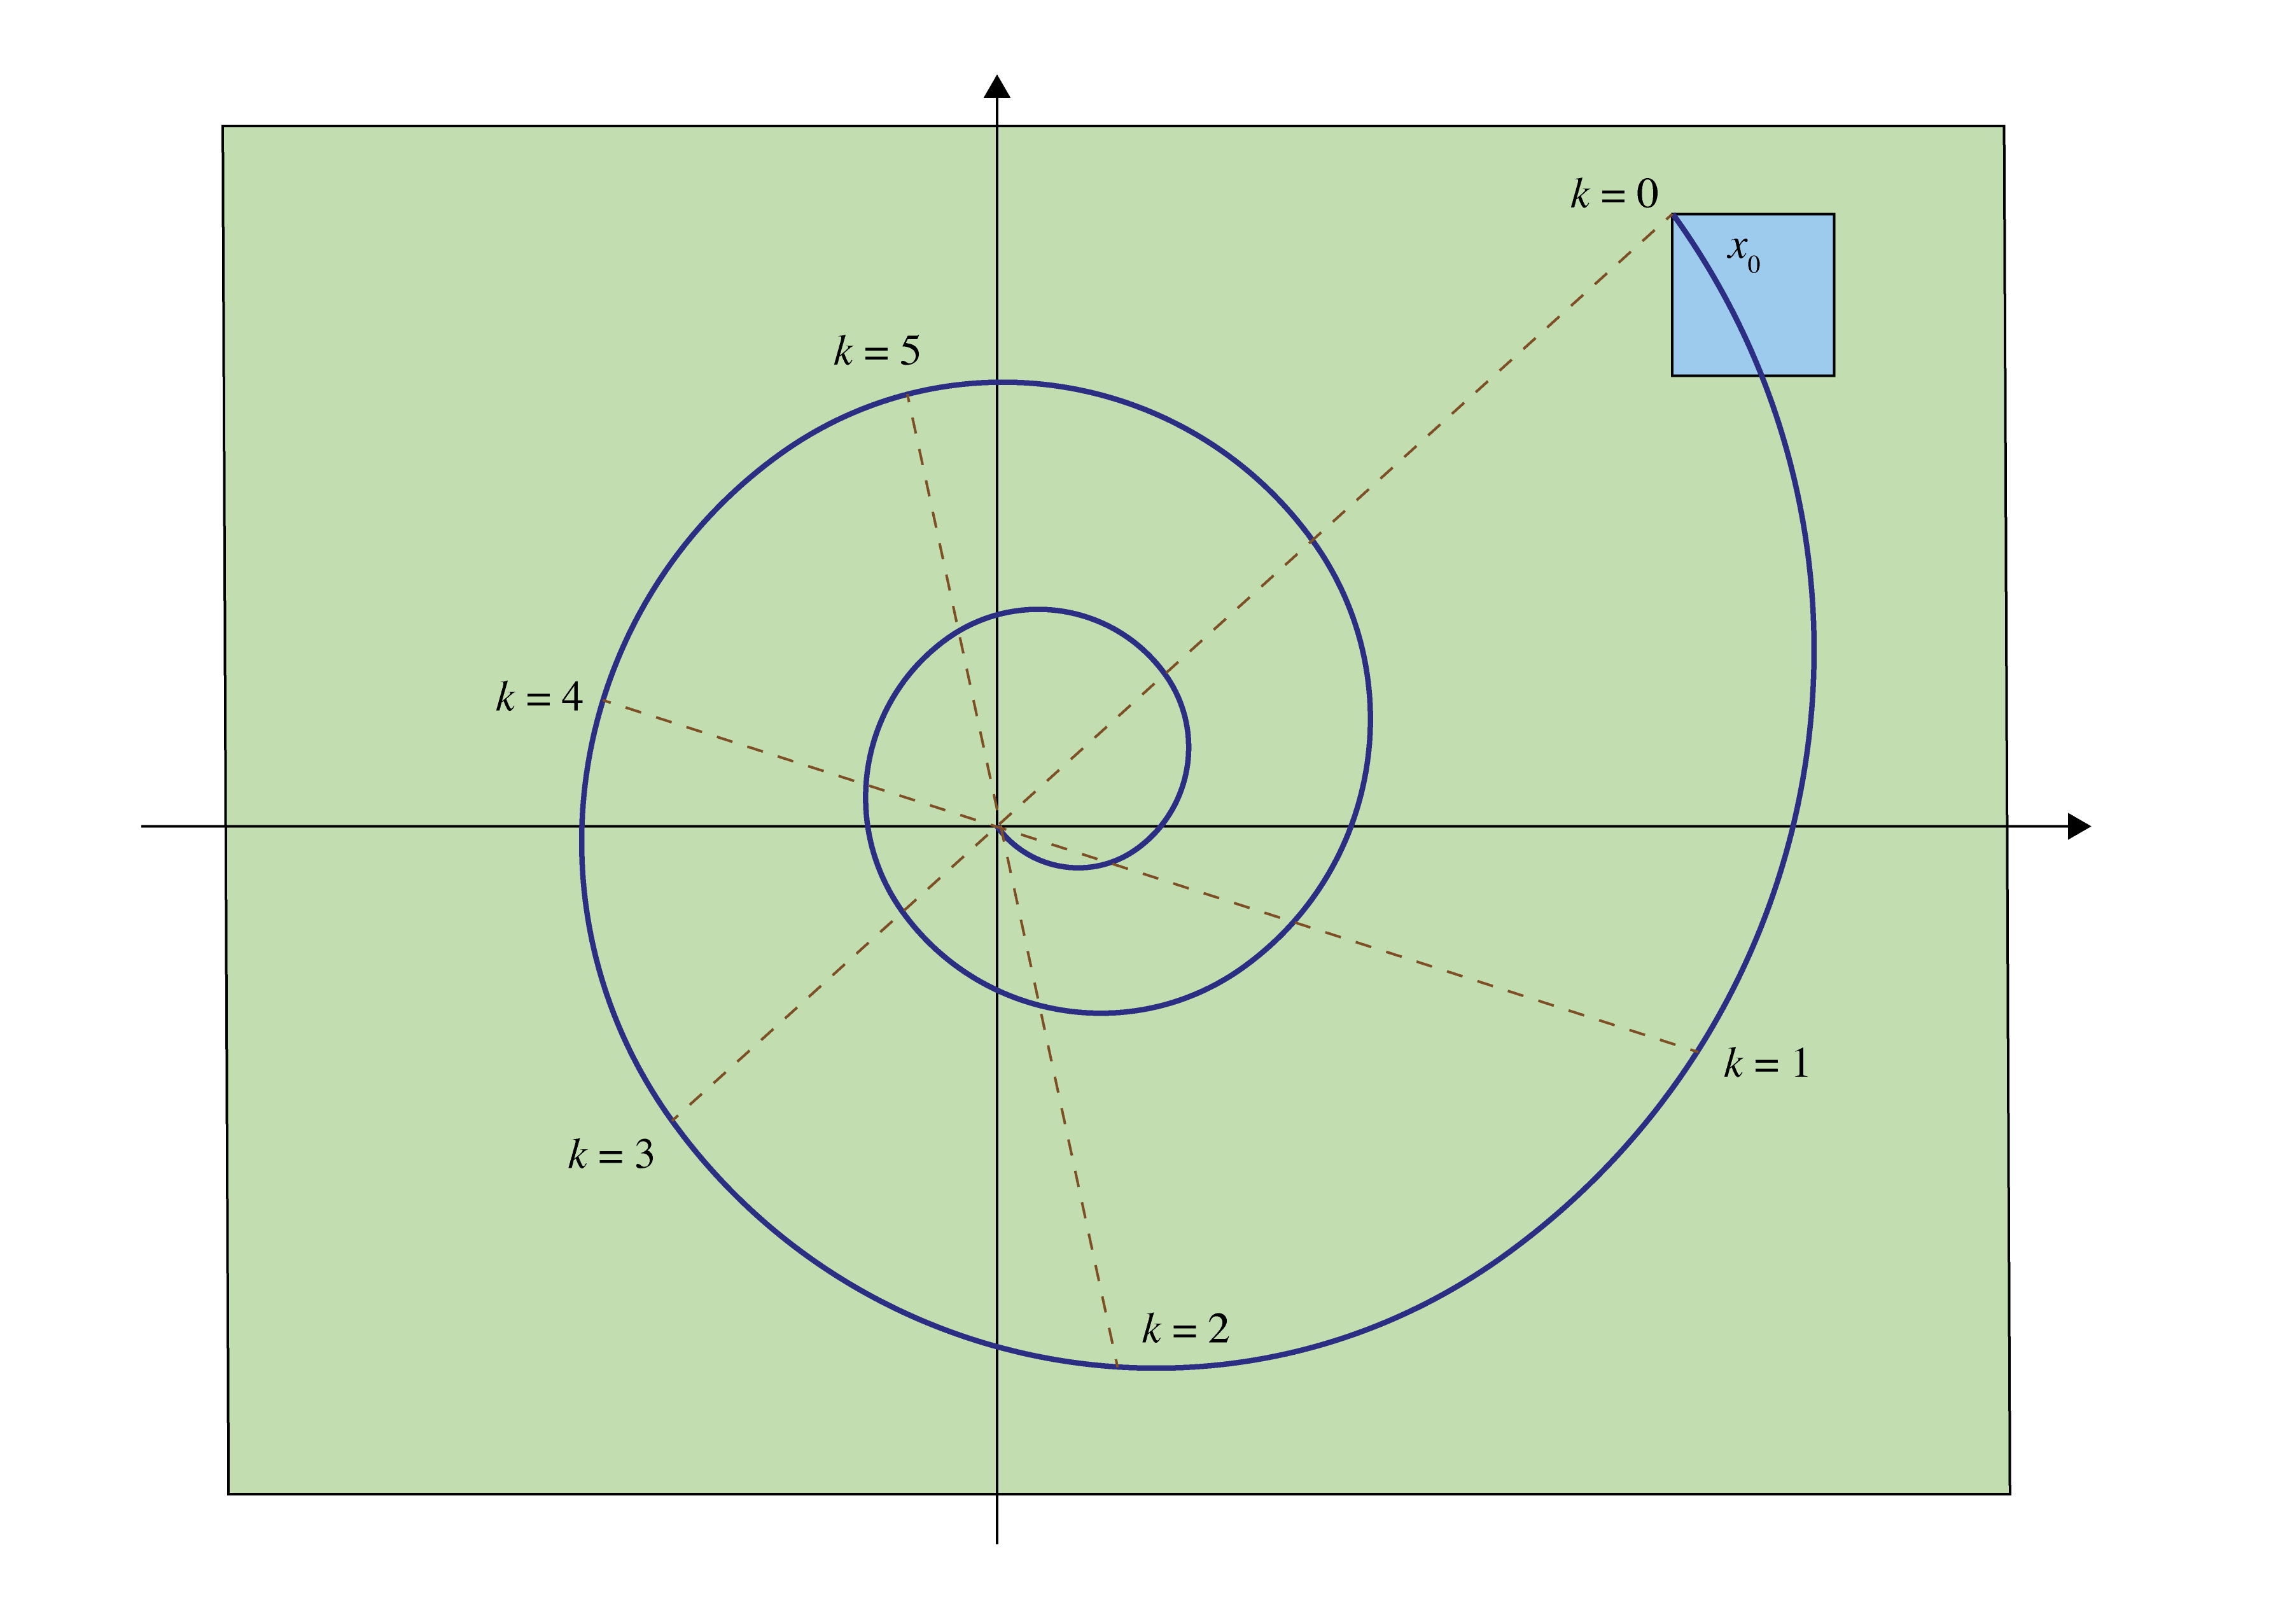
\includegraphics[width=.45\textwidth]{figures/spirals/Spirals-01.png}
%\only<2->{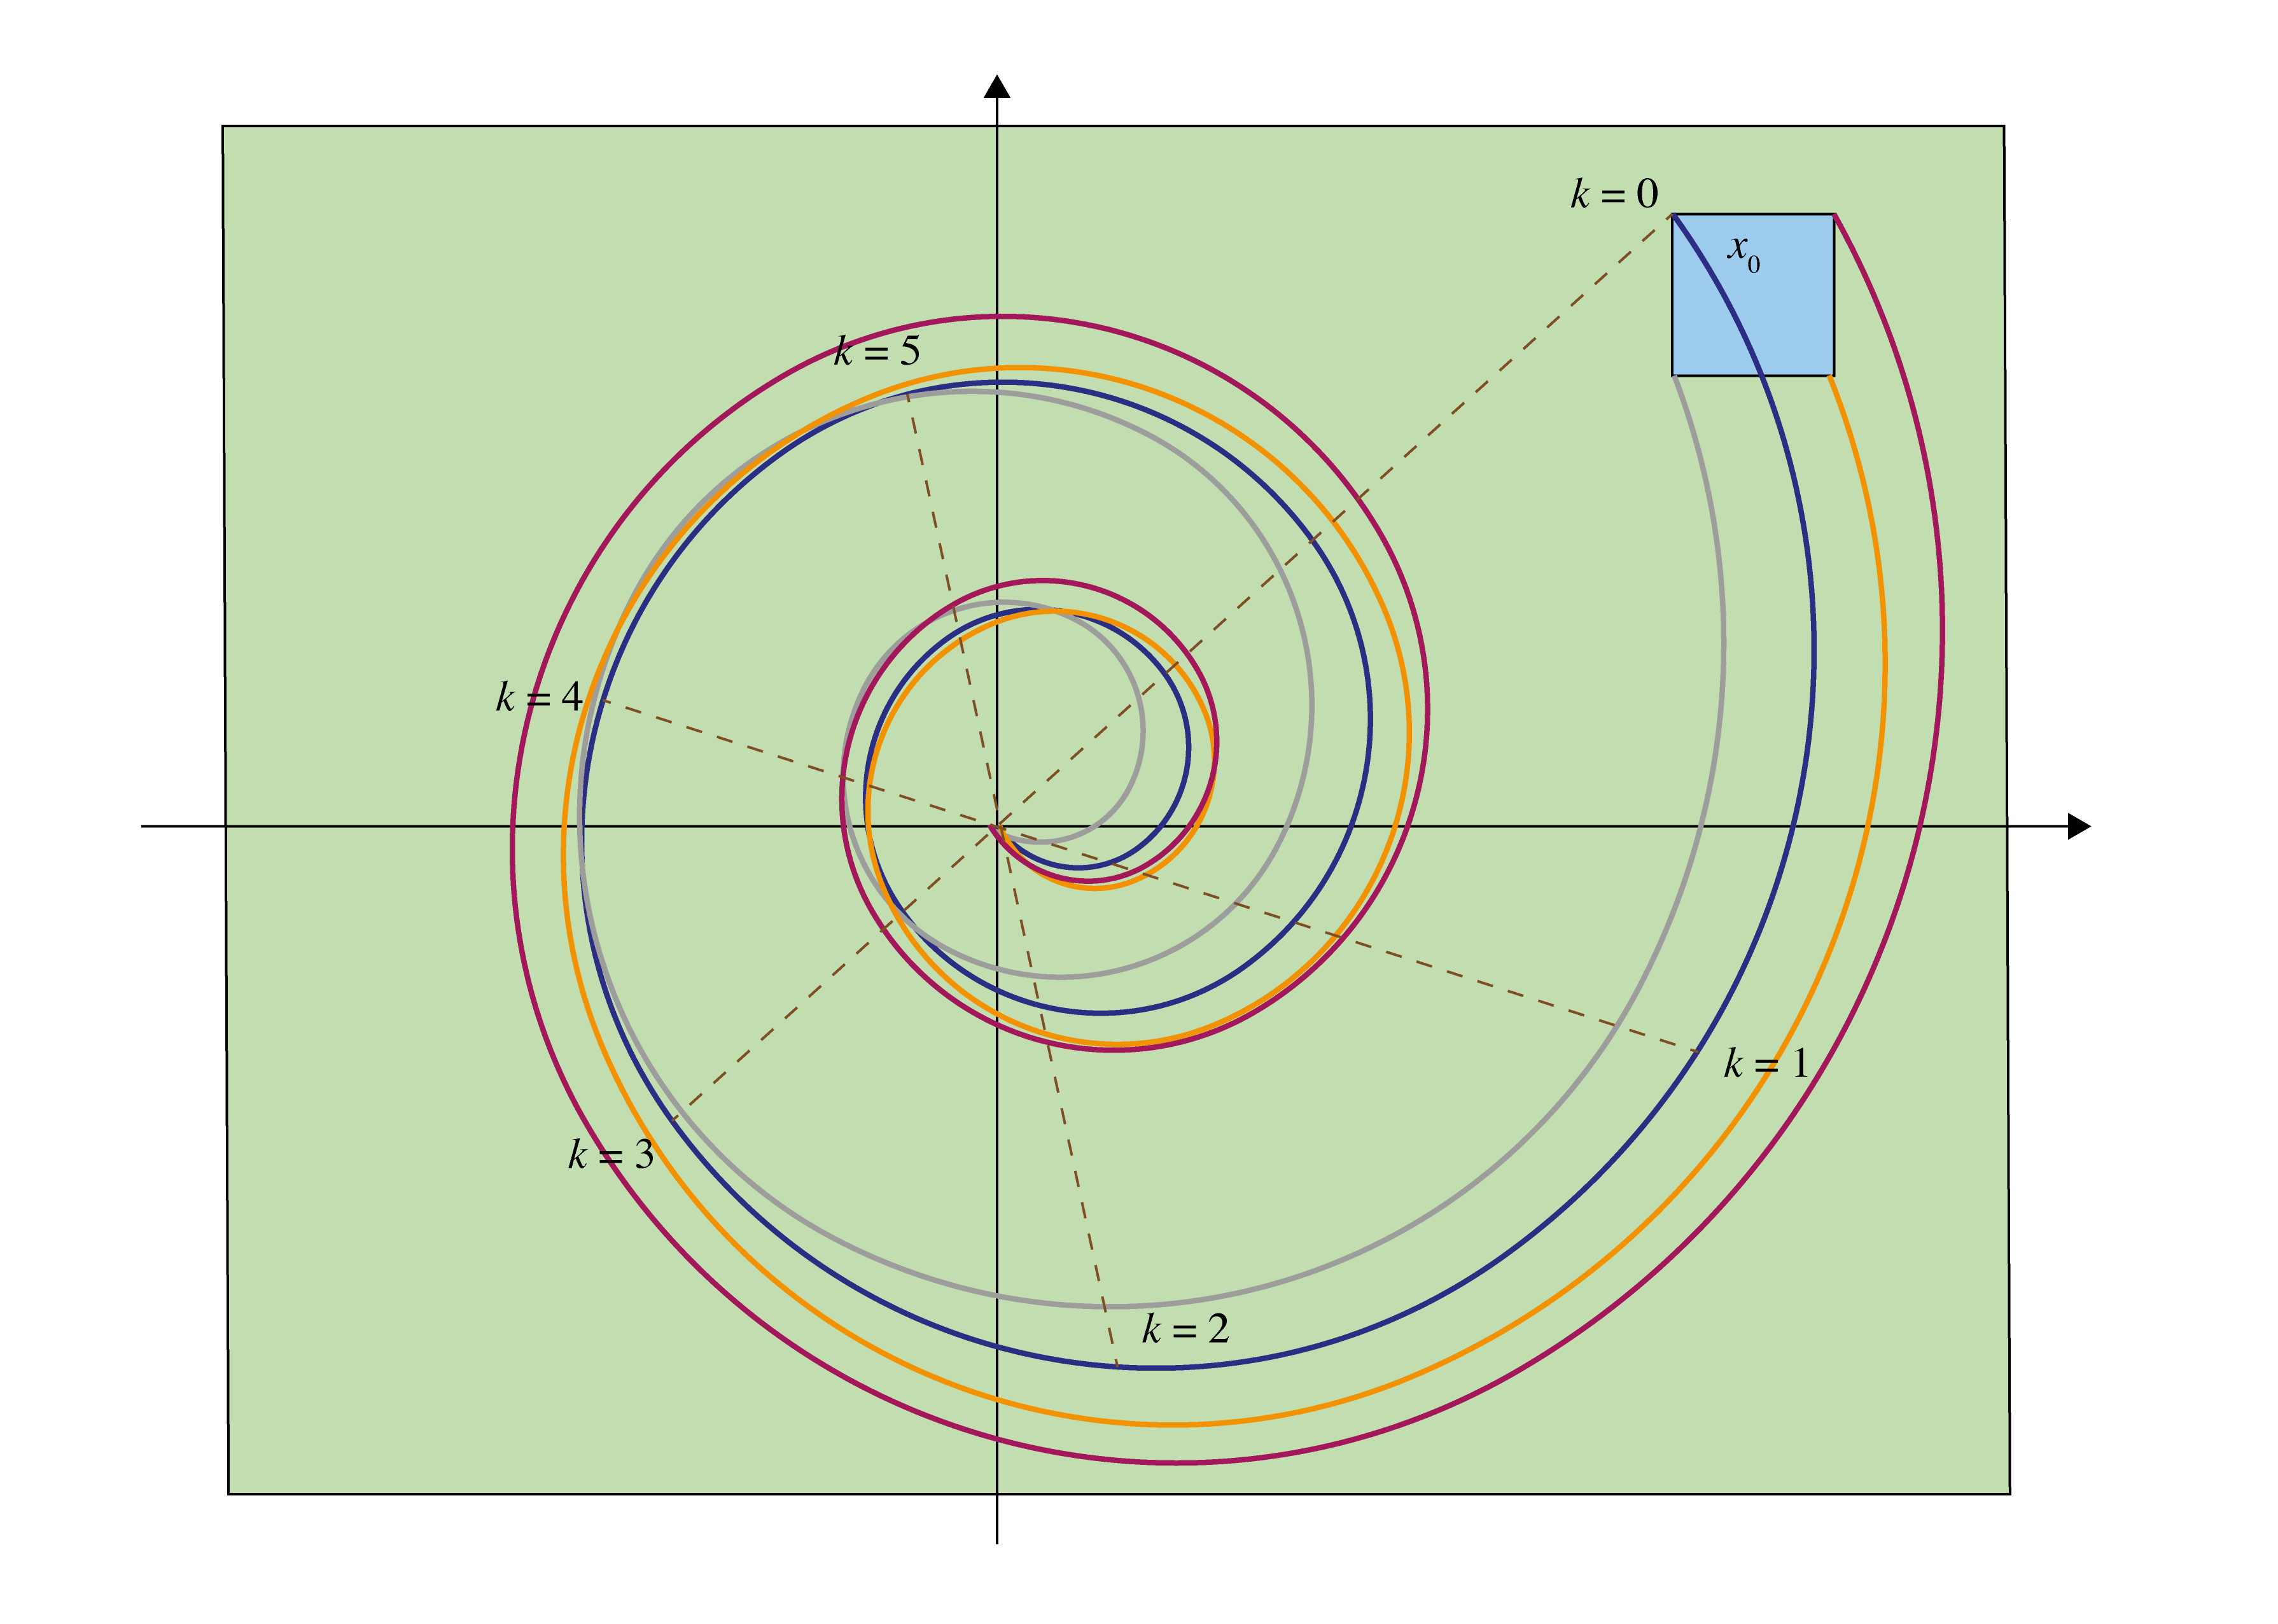
\includegraphics[width=.6\textwidth]{figures/spirals/Spirals-02.png}}
}

% [figure] make initial states square bigger, use a different colour for k.
% first figure: just one spiral
% second figure: 4 spirals

  \end{tabular}
}

\uncover<3->{
  \vspace{.3cm}
{\bf Stability:} Jury's criterion

{\bf Safety:} (1) unwinding up to a completeness threshold (2) abstraction}

%We consider non-deterministic initial states within a
%specified range, the reference signal to be set to zero, saturation on
%the inputs, and account for quantization errors introduced by the
%controller.

%$\exists K. \forall(x_0, u_k). \phi_{stability} \wedge \phi_{safety}$

\end{frame}


\begin{frame}{Completeness threshold-based safety check} %%Na\"ive Approach: CEGIS with multi-staged verification}

%\begin{tabular}{ll}
\vspace{-.5cm}
 \centering 
 {\scriptsize
\resizebox{.65\textwidth}{!}
{
 \begin{tikzpicture}[scale=0.3,->,>=stealth',shorten >=.2pt,auto, semithick, initial text=, ampersand replacement=\&,]
  \matrix[nodes={draw, fill=none, shape=rectangle, minimum height=.2cm, minimum width=.2cm, align=center
},
          row sep=.6cm, column sep=.9cm] {
   \coordinate (aux1);
   \& \coordinate (aux2);
   \&;\\
   \coordinate (aux3);
   \& \coordinate (aux4);
   \&;\\
   \coordinate (aux5);
   \& \coordinate (aux6);
   \&;\\
   \node[minimum width=1.5cm, minimum height=0.6cm, fill=gray!20] (synth) {{\sc 1.Synthesize}};
   \only<2,4>{\node[minimum width=1.5cm, minimum height=0.6cm, fill=red!20] (synth) {{\sc 1.Synthesize}};}
   \&
   complexnode/.pic={ 
     \node[rectangle,draw,dotted,
	minimum width=6cm,
	minimum height=1cm,
        pattern=north west lines, pattern color=gray!20,
	label={\sc ~~~~~~~~~~~~Verify},] (verif) {};
     \node[minimum width=1cm, minimum height=0.6cm, fill=gray!20] (verif1) at ([xshift=-2cm]verif.center) {{\sc 2.Safety}};
     \only<3,5>{\node[minimum width=1cm, minimum height=0.6cm, fill=red!20] (verif1) at ([xshift=-2cm]verif.center) {{\sc 2.Safety}};}
     \node[minimum width=1cm, minimum height=0.6cm, fill=gray!20] (verif2) at ([xshift=0cm]verif.center) {{\sc 3.Precision}};
     \only<6>{\node[minimum width=1cm, minimum height=0.6cm, fill=red!20] (verif2) at ([xshift=0cm]verif.center) {{\sc 3.Precision}};}
     \node[minimum width=1cm, minimum height=0.6cm, fill=gray!20] (verif3) at ([xshift=2cm]verif.center) {{\sc 4.Complete}};
     \only<7>{\node[minimum width=1cm, minimum height=0.6cm, fill=red!20] (verif3) at ([xshift=2cm]verif.center) {{\sc 4.Complete}};}
     %\node[minimum width=1cm, minimum height=0.6cm, fill=gray!20] (verif4) at ([xshift=3.1cm]verif.center) {{\sc 5.Sampling}};
   } 
   \& \node[ellipse, fill=gray!20] (done) {{\sc Done}};
   \only<8>{\node[ellipse, fill=red!20] (done) {{\sc Done}};}\\
   \& \\
   \node[minimum height=0cm] (gp) {\sf Program Search};
   \&
   complexnode/.pic={ 
     \coordinate (aux);
   \node (bmc) at ([xshift=-2cm]aux.center) {\sf BMC-based \\ \sf Verifier};
   \node (fp)  at ([xshift=0cm]aux.center) {\sf Fixed-point \\ \sf Arithmetic\\ \sf Verifier};
   \node (sv)  at ([xshift=2cm]aux.center) {\sf Completeness\\ \sf Verifier};
   %\node (cv)  at ([xshift=3.1cm]aux.center) {\sf Sampling\\Verifier};
   }   
    \\
  };

   \path
    ([yshift=2em]synth.east) edge node[xshift=-0.5em,align=center] {$C$} ([yshift=2em]verif1.west)
    ([yshift=-2em]verif1.west) edge node {C-ex} ([yshift=-2em]synth.east)
    ([xshift=-5em]fp.north) edge node[align=center]  {} ([xshift=-5em]verif2.south)
    ([xshift=-5em]sv.north) edge node[align=center]  {} ([xshift=-5em]verif3.south)
    %([xshift=-5em]cv.north) edge node[align=center]  {T/F} ([xshift=-5em]verif4.south)
    ([xshift=5em]verif1.south) edge node[align=center] {} ([xshift=5em]bmc.north)
    ([xshift=5em]verif2.south) edge node[align=center] {} ([xshift=5em]fp.north)
    ([xshift=5em]verif3.south) edge node[align=center] {} ([xshift=5em]sv.north)
    %([xshift=5em]verif4.south) edge node[align=center] {$C$} ([xshift=5em]cv.north)
    ([xshift=-5em]bmc.north) edge node[align=center]  {} ([xshift=-5em]verif1.south)
    (verif) edge node {PASS} (done)
    ([xshift=5em]synth.south) edge node[align=center] {} ([xshift=5em]gp.north)
    ([xshift=-5em]gp.north) edge node[align=center] {} ([xshift=-5em]synth.south)
    (aux3) edge (synth.north);
   \path[-]
   (verif2.north) edge node[align=center] {} ([xshift=0cm]aux6)
   ([xshift=0cm]aux6) edge node[align=center] {Increase Precision} (aux5)
   (verif3.north) edge node[align=center] {} ([xshift=6.7cm]aux4)
   ([xshift=6.7cm]aux4) edge node[align=center] {Increase Unfolding Bound} (aux3);
   %(verif4.north) edge node[align=center] {} ([xshift=10.5cm]aux2)
   %([xshift=10.5cm]aux2) edge node[align=center] {Increase Sampling Rate} (aux1);

 \end{tikzpicture}
}}

 \scriptsize
 %&
 \begin{tabular}{p{\dimexpr 0.5\linewidth-2\tabcolsep} 
     p{\dimexpr 0.5\linewidth-2\tabcolsep}}

   \only<2>{
     \begin{tabular}{l}
       {\bf Find a controller for given $\{x_0\}$ and $k$} \\
       {\bf such that the system is stable and safe.} \\
%       {\bf states $x_0$, a given number of discrete steps $k$,} \\
 %      {\bf and a given precision $\langle I_p, F_p \rangle$.}\\
     \\\\\\\\\\\\\\\\\\\\\\\\\\
  \end{tabular}
   }
   \only<3>{
     \begin{tabular}{l}
       {\bf Find an initial state for which the system}\\
       {\bf is unsafe.} \\
     %{\bf is stable and safe for all initial states $x_0$.}\\
     %{\bf Use the same $\langle I_p, F_p \rangle$, $k$.}
     \\\\\\\\\\\\\\\\\\\\\\\\\\
  \end{tabular}
   }
   \only<4>{
     \begin{tabular}{l}
       {\bf Find a controller for $\{x_0, x_0'\}$ and $k$}\\
       {\bf such that the system is stable and safe.} \\
%       {\bf states $x_0$, a given number of discrete steps $k$,} \\
 %      {\bf and a given precision $\langle I_p, F_p \rangle$.}\\
     \\\\\\\\\\\\\\\\\\\\\\\\\\
  \end{tabular}
   }
   \only<5>{
     \begin{tabular}{l}
       {\bf Find an initial state for which the system}\\
       {\bf is unsafe.} \\       
     %% {\bf Verify that the closed-loop system} \\
     %% {\bf is stable and safe for all initial states $x_0$.}\\
     %% {\bf Use the same $\langle I_p, F_p \rangle$, $k$.}
     \\\\\\\\\\\\\\\\\\\\\\\\\\     
  \end{tabular}
   }
   \only<6>{
     \begin{tabular}{l}
     {\bf Check that the plant precision is sufficient.}\\
     \\\\\\\\\\\\\\\\\\\\\\\\\\\\     
  \end{tabular}
   }
   \only<7>{
     \begin{tabular}{l}
       {\bf Check that $k$ is sufficient.} \\
     \\\\\\\\\\\\\\\\\\\\\\\\\\\\     
  \end{tabular}
   }
   \only<8>{
     \begin{tabular}{l}
       {\bf Controller found.}\\
     \\\\\\\\\\\\\\\\\\\\\\\\\\\\     
  \end{tabular}
   }
 
   &
%\adjustbox{valign=t}{  
 \only<2>{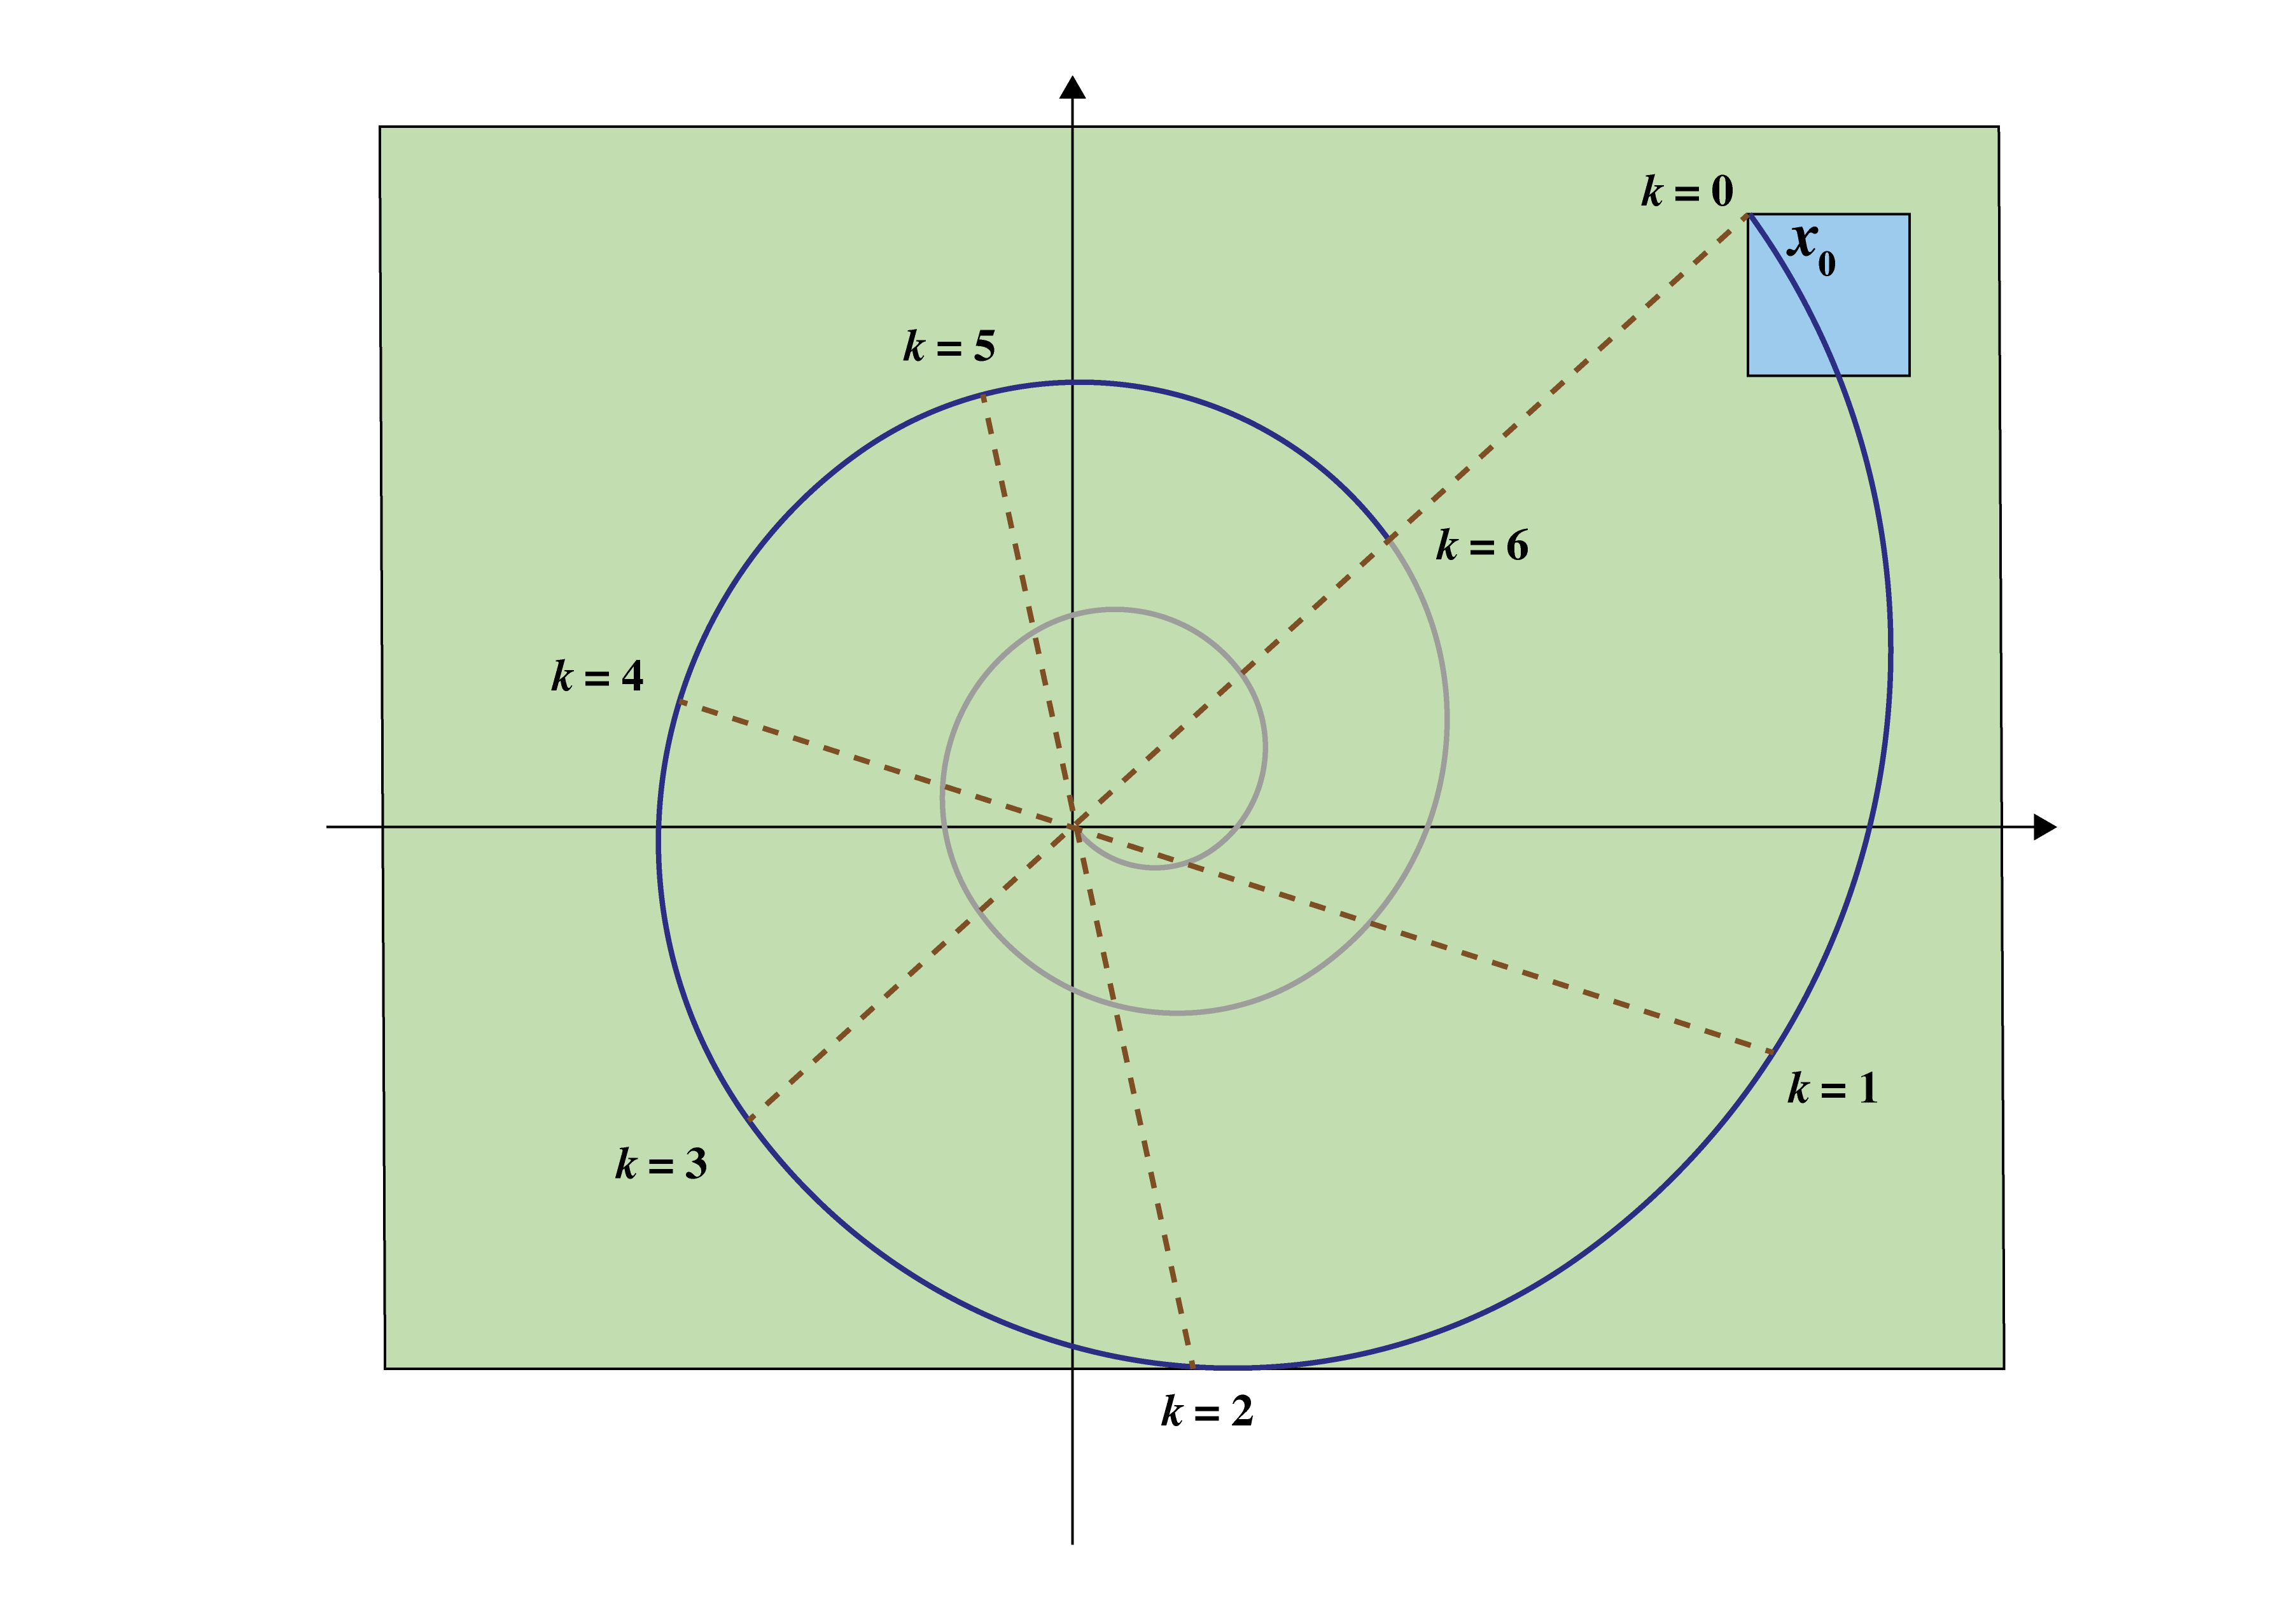
\includegraphics[width=.55\textwidth]{figures/spirals/Spirals-05.png}}
 \only<3>{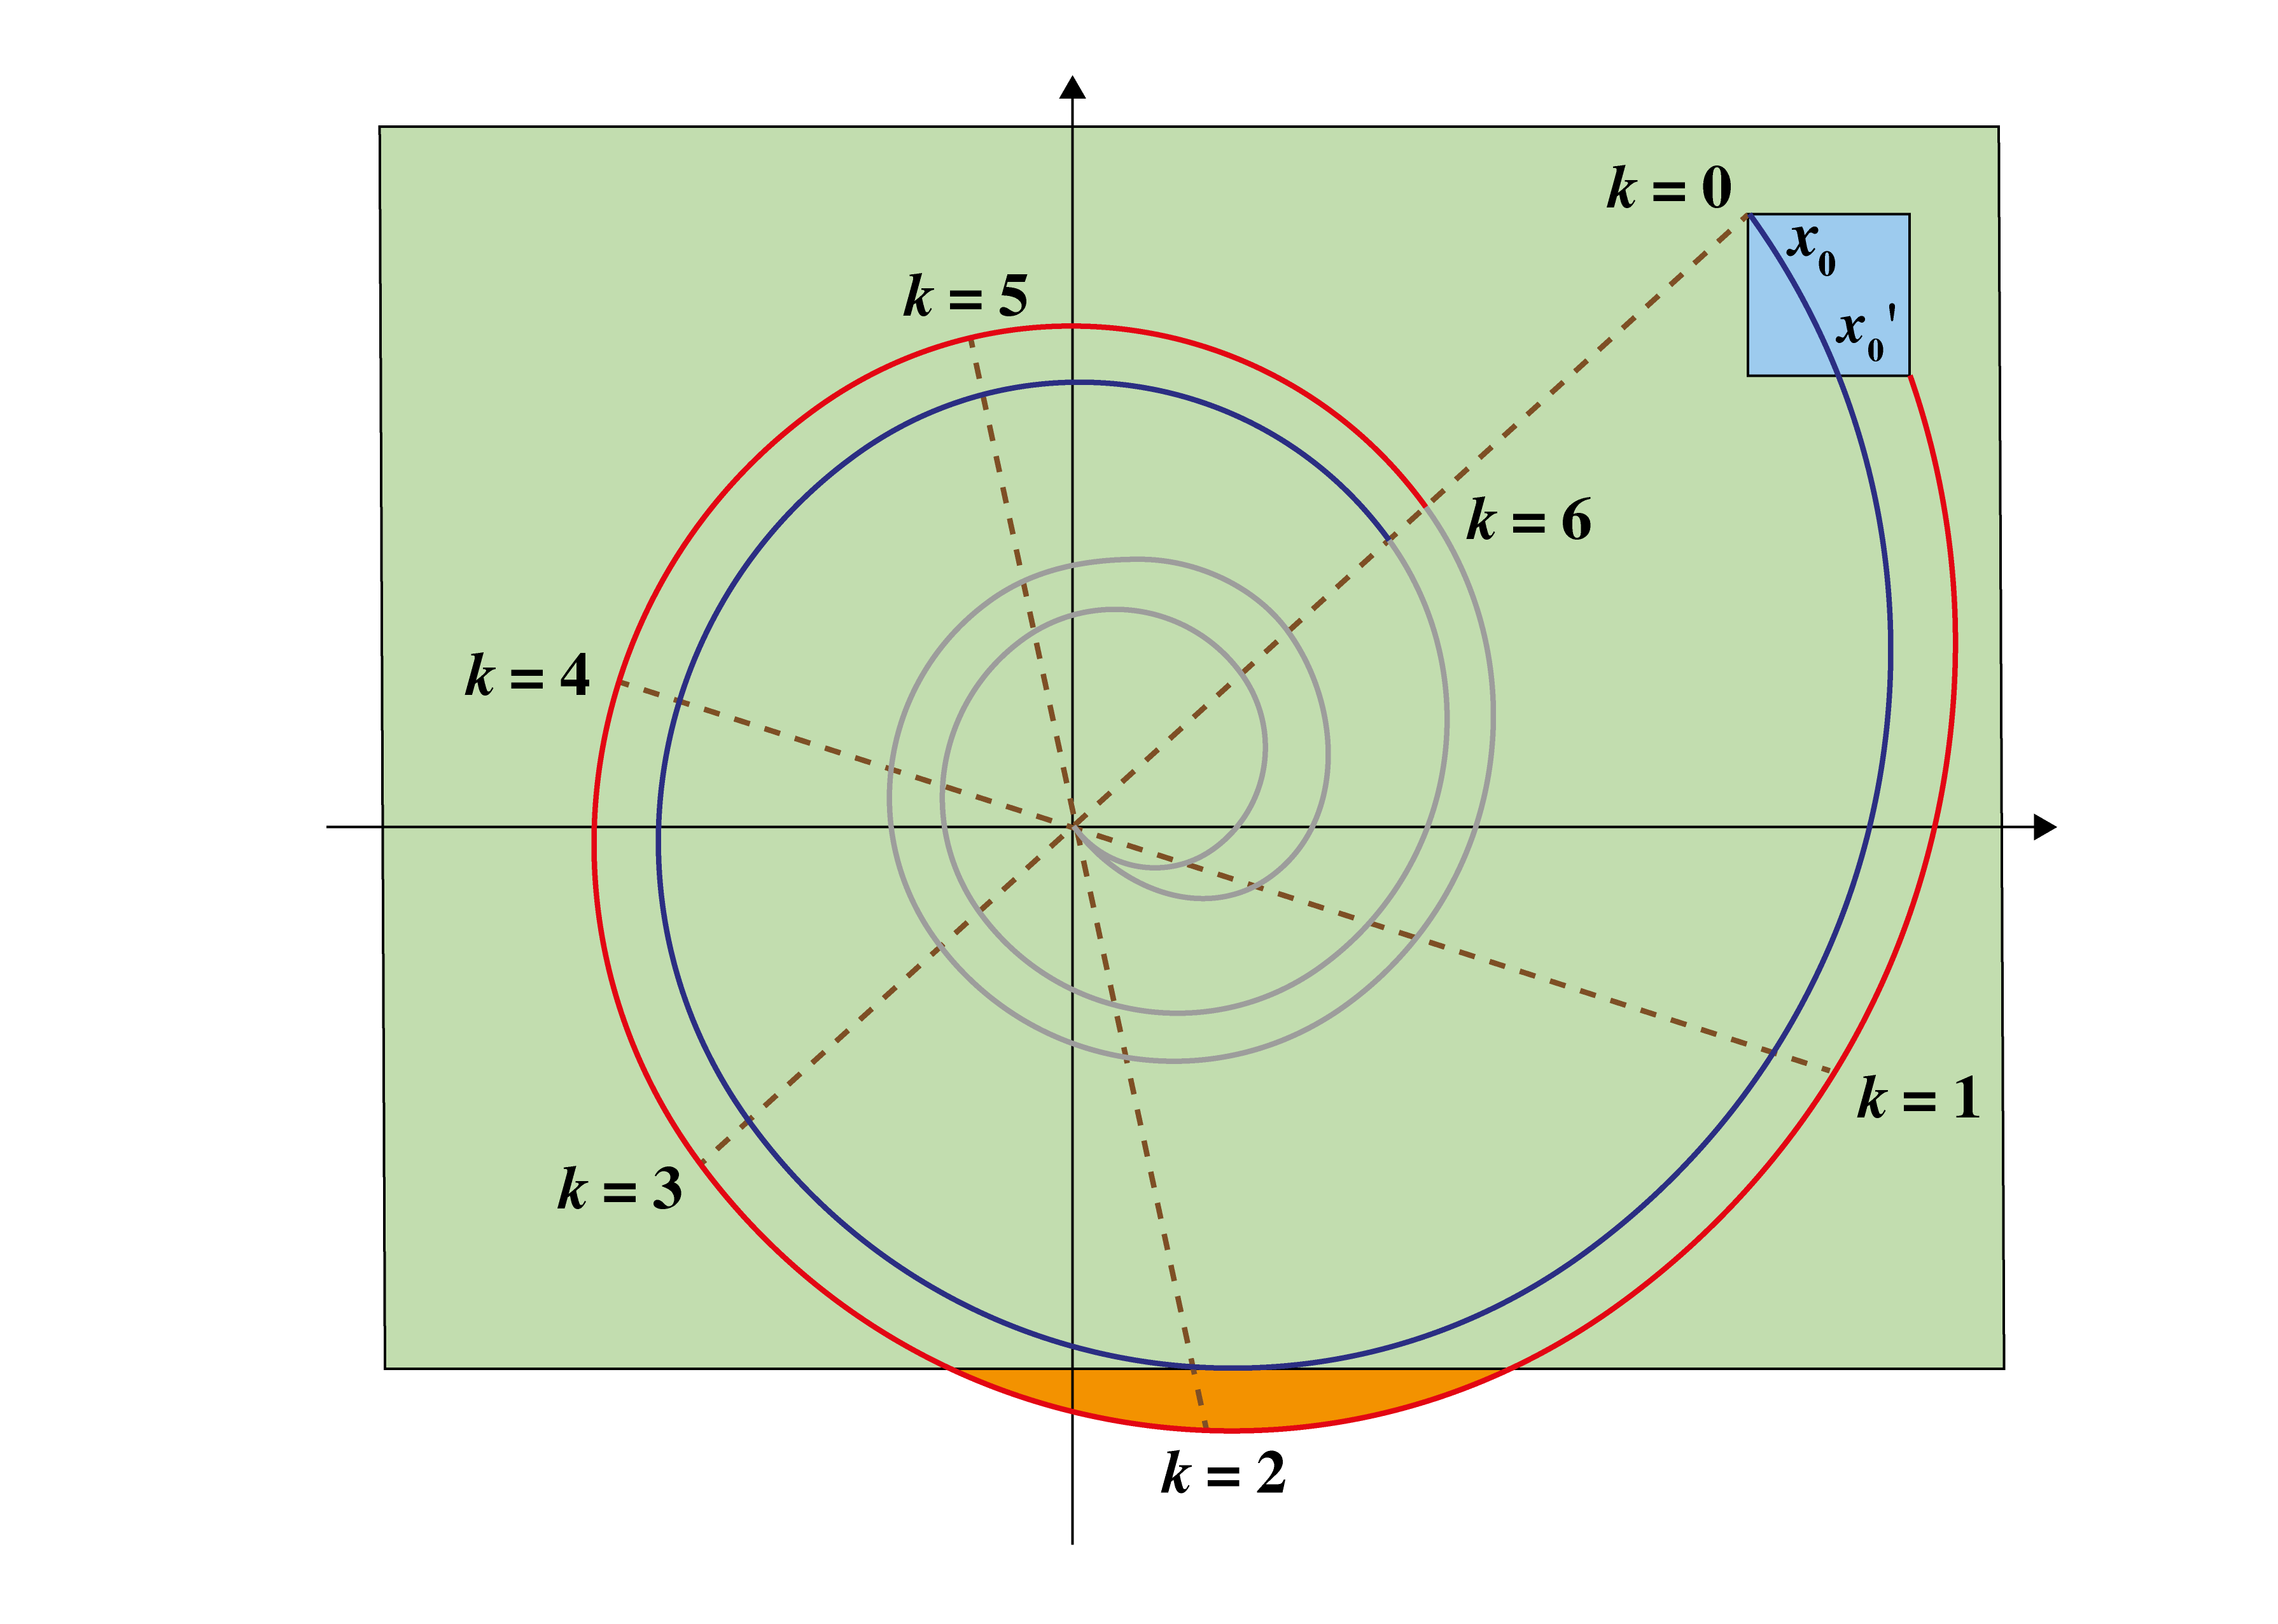
\includegraphics[width=.55\textwidth]{figures/spirals/Spirals-04.png}}
 \only<4,5,6>{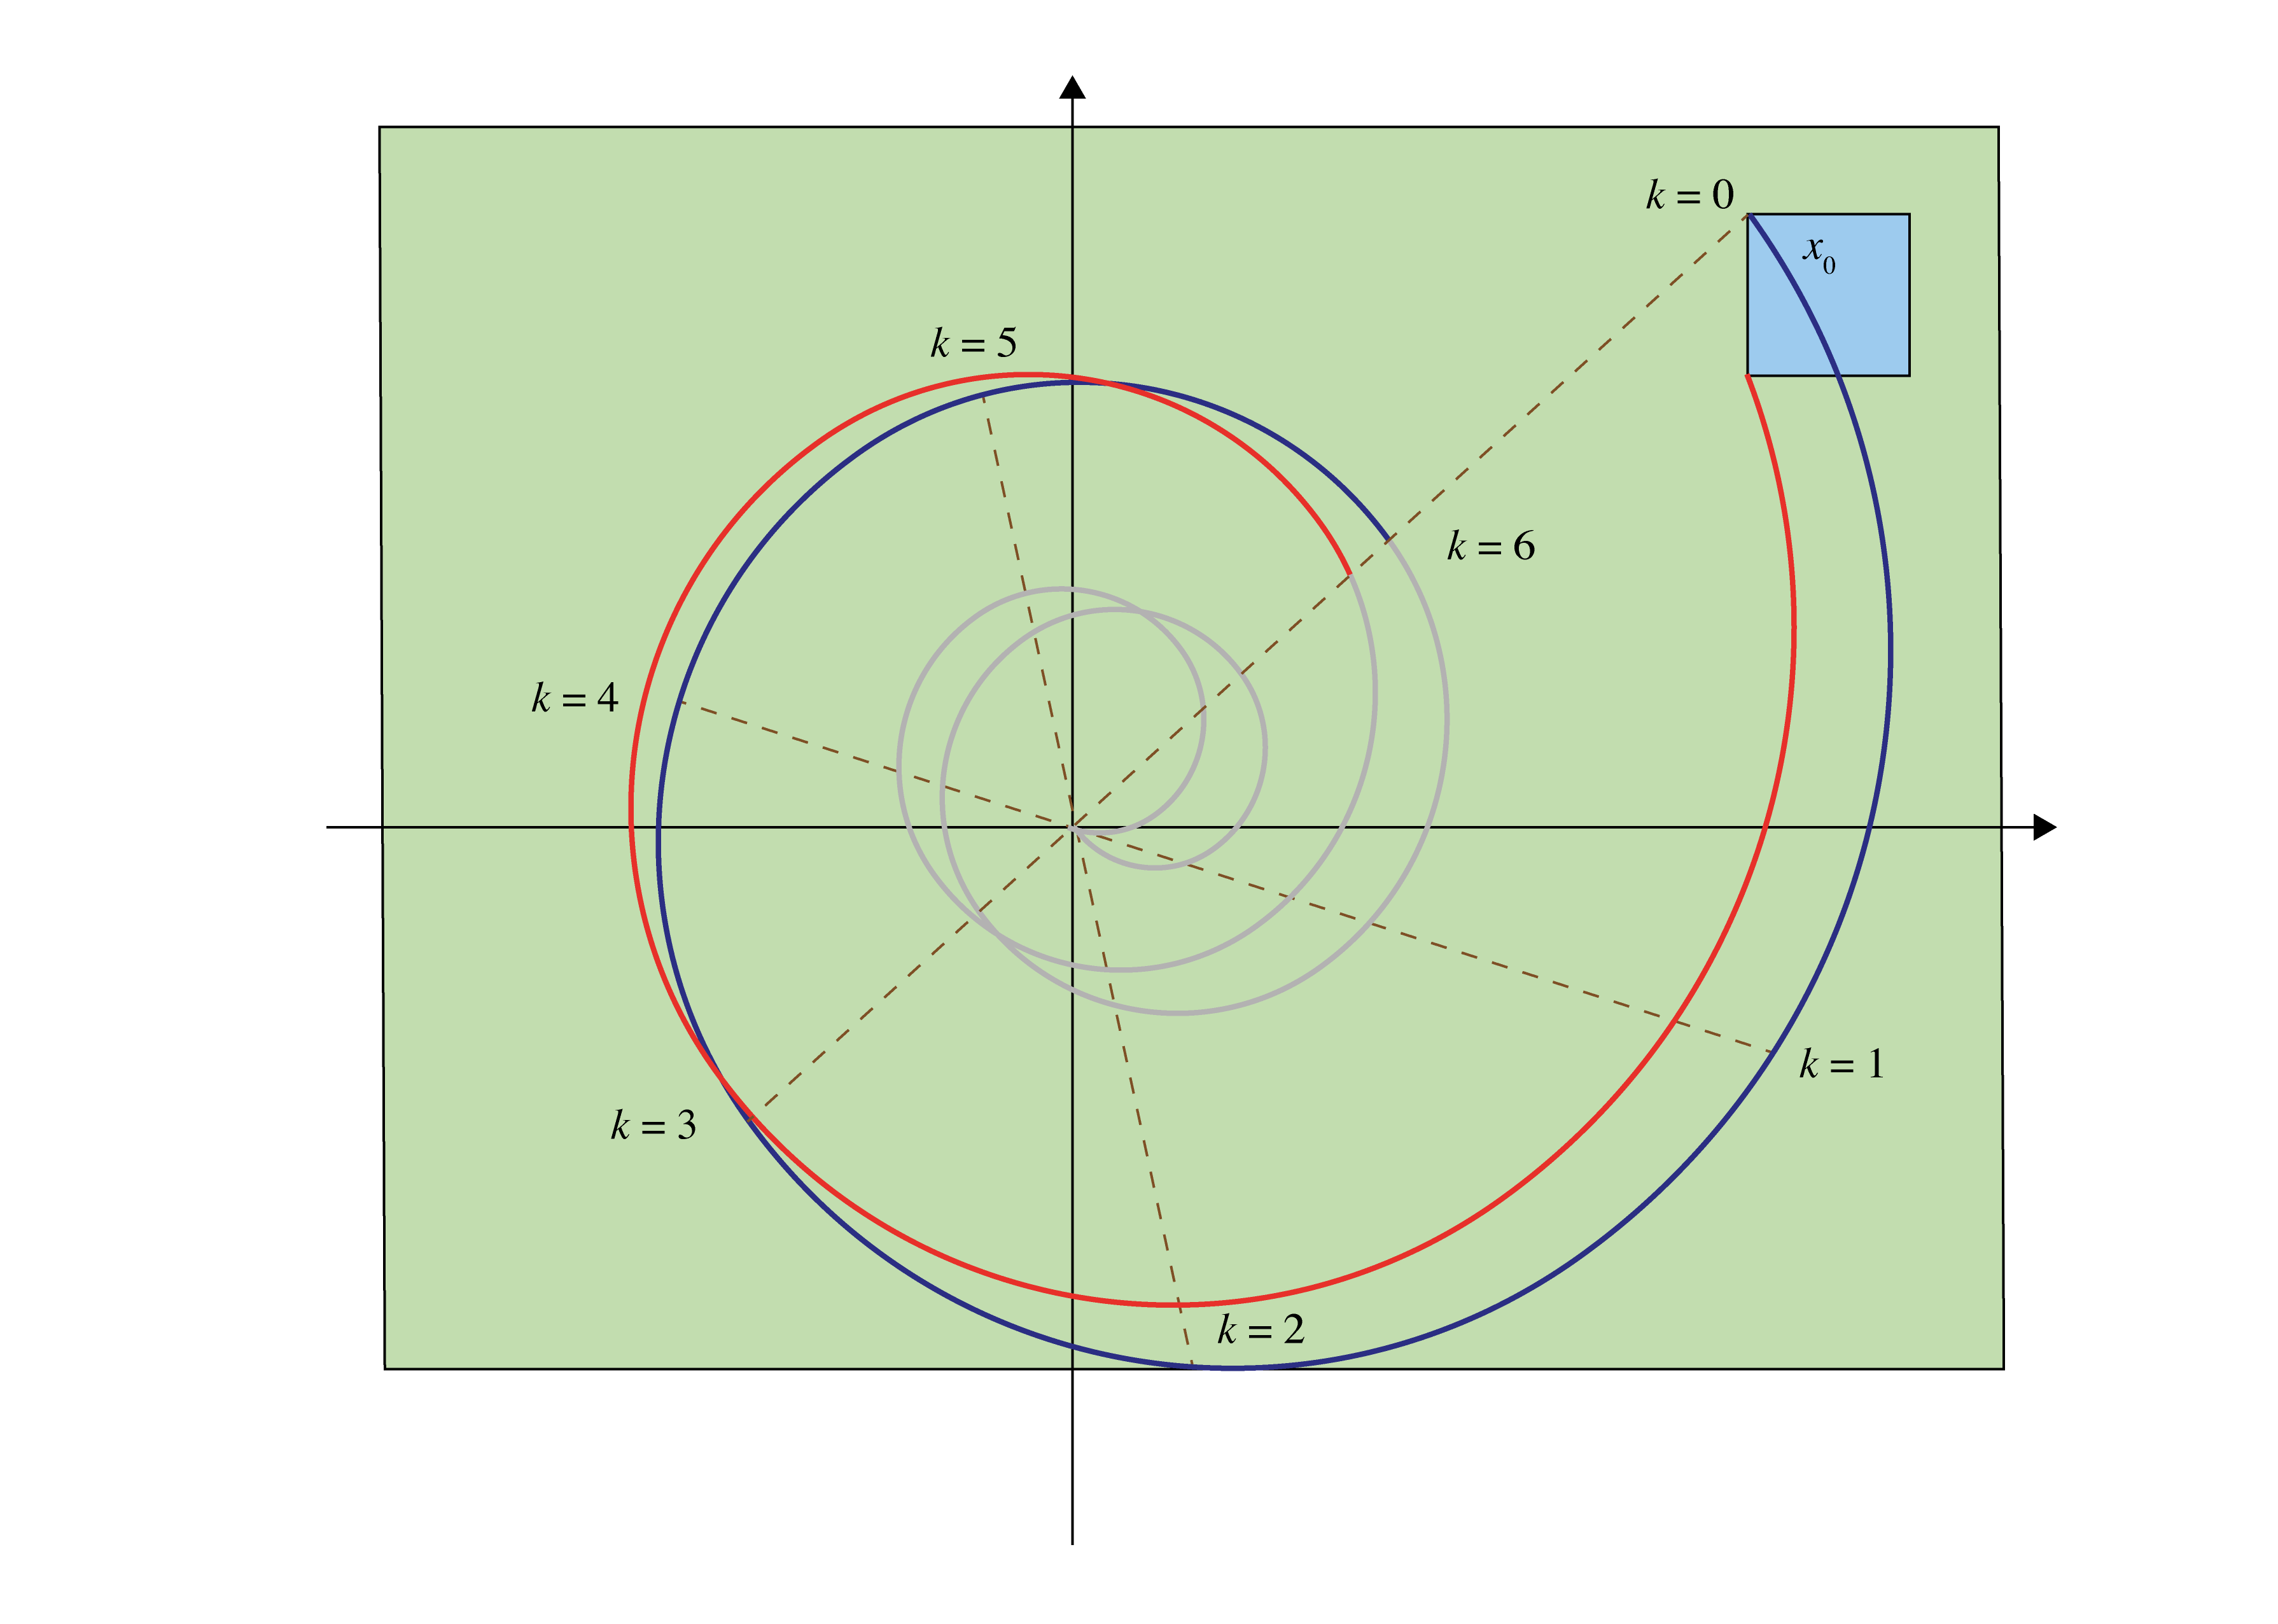
\includegraphics[width=.55\textwidth]{figures/spirals/Spirals-06.png}}
 \only<7->{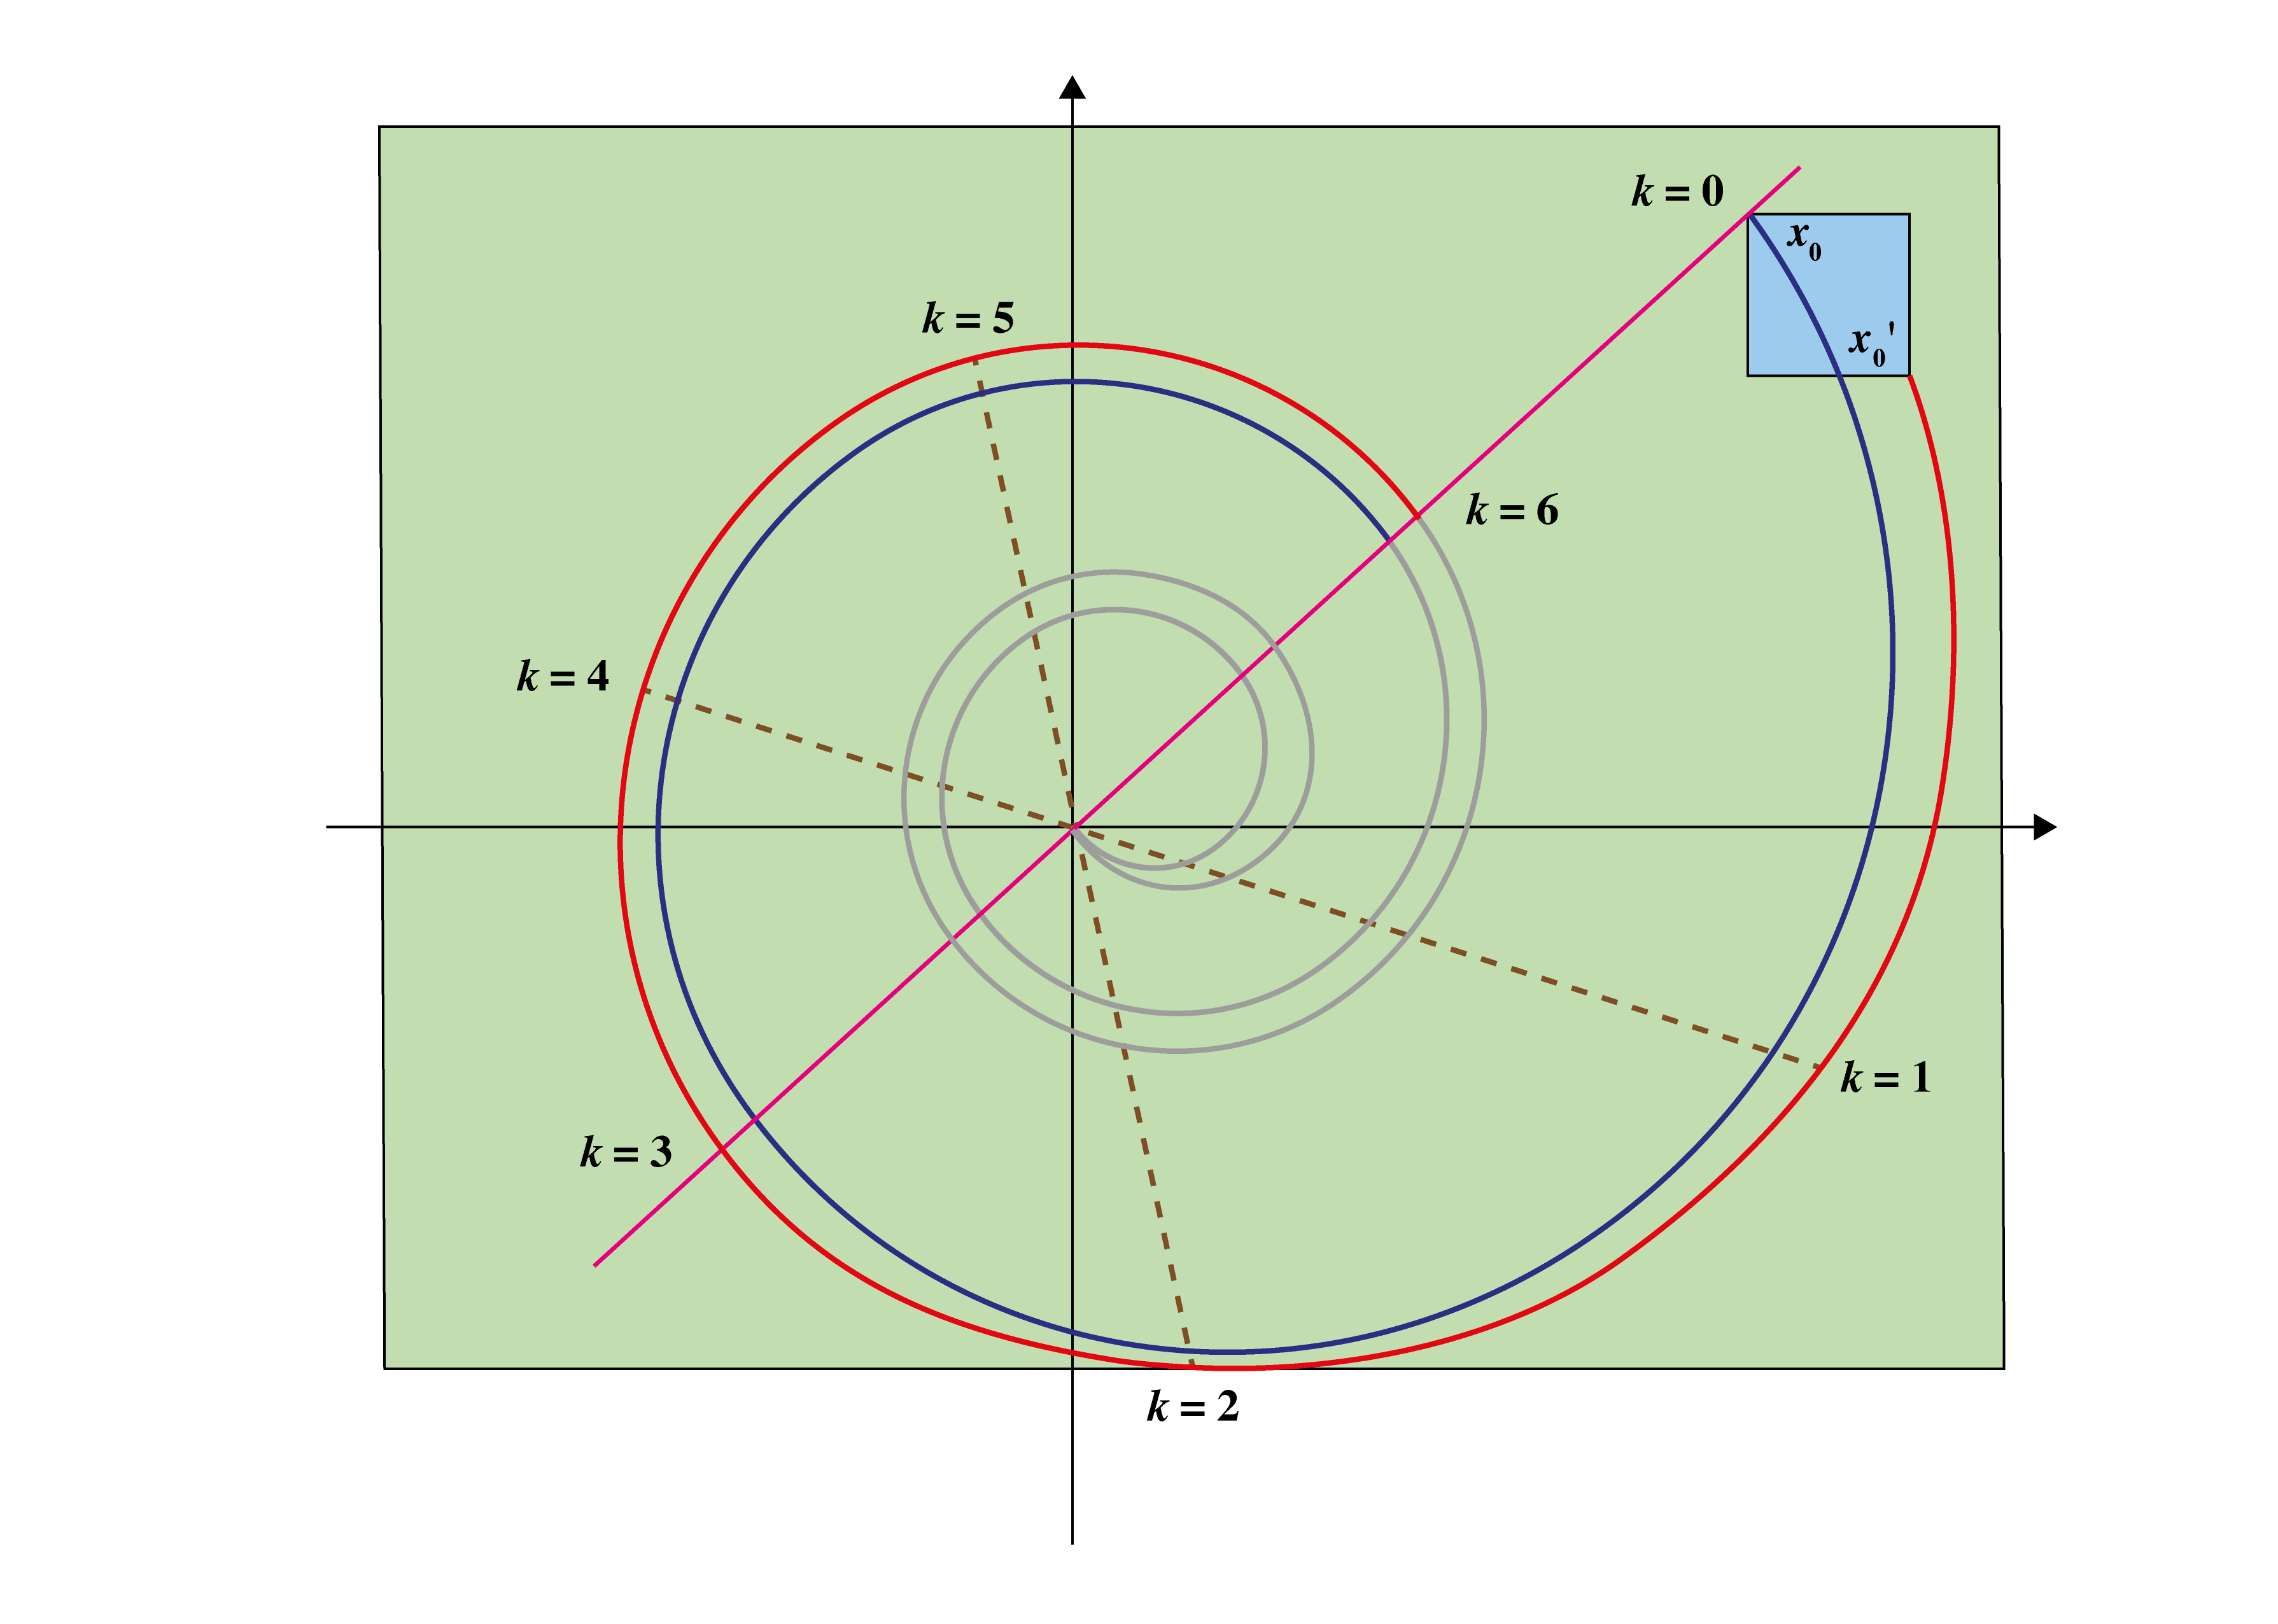
\includegraphics[width=.55\textwidth]{figures/spirals/Spirals-06-prime.png}}   
%}
\end{tabular}

 %[figure]: Re-draw such that the spiral doesn't reach the origin.
 % second figure for safety: put all the 4 incomplete spirals in.
 % for the completeness threshold: complete the spiral with
 % dashed line.
\end{frame}


%% \begin{frame}{Na\"ive Approach: CEGIS with multi-staged verification}

%% \begin{itemize}  
%% \item Synthesis: get a controller that is stable and safe for an initial state,
%%   plants precision, completeness threshold and sampling rate.

%% \item Verification:
%%   \begin{itemize}
%% \item First stage: verify the controller is safe for all initial states.
%% performs potentially unsound fixed-point operations
%% assuming a plant precision $\langle I_p,F_p \rangle$.

%% \item The second stage restores soundness with respect to the plant's precision
%% by using interval arithmetic on the synthesized controller.

%% \item The third stage: check that we are above the completeness threshold.
%%   \end{itemize}
%% \end{itemize}

%% {\bf Observation:} Checking that the safety specification holds for
%% any initial state can be computationally expensive if the bounds on
%% the allowed initial states are large.
%% If a controller is safe for each of the corner cases of our hypercube of
%% allowed initial states, it is safe for any initial state in the hypercube. 

%% \end{frame}

%% \begin{frame}{Na\"ive Approach: CEGIS with multi-staged verification}
%%   Synthesizes a controller for an individual initial state and input with a
%%   bounded time horizon and, subsequently,
%% it generalizes it to all reachable states, inputs, and time horizons during the
%% verification phase.
%% \end{frame}

%% \begin{frame}{Abstraction-based approach}
%% Find a controller for a continuous initial set of states and set of
%% inputs, over an abstraction of the continuous dynamics.

%% We use an abstraction of the continuous dynamics that confirms to
%% witness proofs at specific times.

%% We use abstract acceleration to compute the reach-tube $\hat{X}^\#$, i.e. the set of all
%% reachable states at all given times given an initial set $\phi_{init}$.

%% \end{frame}



\begin{frame}{Experimental results}
  
\begin{table}
\centering
\scriptsize
\begin{tabular}{| r | l | c | c | r | c | r |}
%
\hline
\# & \multicolumn{1}{|c|}{Benchmark} & \multicolumn{1}{|c|}{Order} & \multicolumn{2}{|c|}{Completeness threshold}                 & \multicolumn{2}{|c|}{Abstraction} \\
   &                                  & & \multicolumn{1}{|c|}{$\langle I_p,F_p \rangle$} & \multicolumn{1}{|c|}{Time} & \multicolumn{1}{|c|}{$\langle I_p,F_p \rangle$} & \multicolumn{1}{|c|}{Time} \\\hline
1  & {\bf Cruise Control}  & 1 & \cellcolor{green!40}8,16   & \cellcolor{green!40}8.40\,s & 16,16  &    2.17\,s \\
2  & {\bf DC Motor}          & 2 & \cellcolor{green!40}8,16   & \cellcolor{green!40}9.45\,s & 20,20  &   2.06\,s \\
3  & {\bf Helicopter}        & 3 & \cellcolor{red!40}\xmark &  \cellcolor{red!40}\xmark  & 16,16  &    1.37\,s \\
4  & {\bf Inverted Pendulum} & 4 & \cellcolor{green!40}8,16   & \cellcolor{green!40}9.65\,s & 16,16  &    0.56\,s \\
5  & {\bf Magnetic Pointer}  & 2 & \cellcolor{red!40}\xmark &  \cellcolor{red!40}\xmark  & 28,28  &   44.14\,s \\
6  & {\bf Magnetic Suspension} & 2 & \cellcolor{green!40}12,20  & \cellcolor{green!40}10.41\,s & 16,16  &    0.61\,s \\
7  & {\bf Pendulum}          & 2 & \cellcolor{green!40}8,16   & \cellcolor{green!40}14.02\,s & 16,16  &    0.60\,s \\
8  & {\bf Suspension}        & 2 & \cellcolor{green!40} 12,20  & \cellcolor{green!40}73.66\,s & \xmark &    \xmark \\
9  & {\bf Tape Driver}       & 3 & \cellcolor{green!40}8,16   & \cellcolor{green!40}10.10\,s & 16,16  &  68.24\,s \\
10 & {\bf Satellite}          & 2 & \cellcolor{green!40}8,16   & \cellcolor{green!40}9.43\,s & 16,16  &  0.67\,s \\\hline
%
\end{tabular}
\end{table}

Timeout = 1 hour

\end{frame}

%% \begin{frame}{Experimental results}
%% For the majority of our benchmarks, the abstraction-based back-end is
%% faster than the basic multi-staged verification approach, and finds
%% one solution more.

%% The two back-ends complement each other in benchmark coverage and
%% together solve all benchmarks in the set.

%% On average our engine spent 52\% in the synthesis and 48\% in the
%% verification phase.

%% %% There are a few instances for which the system fails to find a controller. 
%% %% For the na\"ive approach, the completeness threshold may be too large, thus
%% %% causing a timeout.  On the other hand, the abstraction-based approach may
%% %% require a very precise abstraction, resulting in too many refinements and,
%% %% consequently, in a timeout.  Yet another source of incompleteness is the
%% %% inability of the {\sc synthesize} phase to use a large enough precision for
%% %% the plant model.


%% \end{frame}

\begin{frame}{Conclusions}

We built an {\bf automated synthesizer for digital state-feedback
controllers} that ensures both {\bf stability} and {\bf safety}.
%over the state-space representation.

\vspace{1cm}

We considered the errors caused 
by the implementation of the digital control algorithm and the
modeling of plant dynamics.

\end{frame}  


\begin{frame}{Abstraction-based controller synthesis}
\vspace{-1cm}
\resizebox{.9\textwidth}{!}
{
\centering
{\scriptsize
  \begin{tikzpicture}[scale=0.3,->,>=stealth',shorten >=.2pt,auto, semithick, ampersand replacement=\&,]
  \matrix[nodes={draw, fill=none, shape=rectangle, minimum height=.2cm, minimum width=.2cm, align=center},row sep=1.5cm, column sep=2cm] {
   \coordinate (aux1);
   \& \coordinate (aux2);
   \& ;\\
   %\& \node[fill=gray!20,align=center] (abstract) {\sc 4. abstract};
   %\& \coordinate (aux); \\ 
   \& \node[fill=gray!20,align=center] (synth) {\sc 2. synthesize};
    \only<2,7>{\node[fill=red!20,align=center] (synth) {\sc 2. synthesize};}   
   \& \node[fill=gray!20,align=center, minimum width=3.5cm] (verify) {\sc 3. verify };
   \only<3,6,8,10>{\node[fill=red!20,align=center, minimum width=3.5cm] (verify) {\sc 3. verify ($\phi$)};}
   \& \node[ellipse, fill=gray!20] (done) {{\sc Done}};
   \only<10>{\node[ellipse, fill=red!20] (done) {{\sc Done}};}\\   
   \& \node[draw,rectangle,align=center] (KSAT) {Program \\ Search};
   \& complexnode/.pic={
     \coordinate (AA);
     \node[draw,rectangle,align=center] (AAV) at ([xshift=-1.5cm]AA.center) {Abstract\\Acceleration};
     \only<3,5,8>{\node[draw,fill=red!20,rectangle,align=center] (AAV) at ([xshift=-1.5cm]AA.center) {Abstract\\Acceleration};}
     \node[draw,rectangle,align=center] (AAC) at ([xshift=1.5cm]AA.center) {Abstraction \\ Verifier};
     \only<4,6,9>{\node[draw,fill=red!20,rectangle,align=center] (AAC) at ([xshift=1.5cm]AA.center) {Abstraction \\ Verifier};}
   }
   \& \\   
  };
  %\path (abstract.south) edge node{$\textcolor{blue}{\begin{array}{c}\phi_{init}^K\\P_a(z)\\k=0\end{array}}$} (synth.north);
    \path ([yshift=1em]synth.east) edge node {$C$} ([yshift=1em]verify.west);
    \path ([yshift=-1em]verify.west) edge node{$(k, x_0)$} ([yshift=-1em]synth.east);
    %\path (aux) edge (abstract.east);
    \path(verify.east) edge (done.west);

  \path ([xshift=+.6cm]KSAT.north) edge[left] node[xshift=-.3cm] {} ([xshift=0.6cm]synth.south);
   \path ([xshift=-.6cm]synth.south) edge node[align=center,xshift=.3cm] {} ([xshift=-.6cm]KSAT.north);
    \path ([yshift=.5cm]AAV.east) edge node{\sl $\hat{X}$} ([yshift=.5cm]AAC.west);
    \path ([yshift=-.5cm]AAC.west) edge node{} ([yshift=-.5cm]AAV.east);
    \path (AAC.north) edge node{} ([xshift=4.9cm]verify.south);
    \path ([xshift=-5cm]verify.south) edge node{$C$} (AAV.north);

\end{tikzpicture}
}}


 \scriptsize
 %&
 \begin{tabular}{p{\dimexpr 0.5\linewidth-2\tabcolsep} 
     p{\dimexpr 0.5\linewidth-2\tabcolsep}}

   \only<2>{
     \begin{tabular}{l}
       {\bf Find controller for given $\{x_0\}$ and $\{k\}$}\\
       {\bf such that the system is stable and safe.}
     \\\\\\\\\\\\\\\\\\\\\\\\\\\\\\
  \end{tabular}
   }
   \only<3>{
     \begin{tabular}{l}
     {\bf Use abstract acceleration to compute an} \\
     {\bf overapproximation the set of all reachable}\\
     {\bf states at all times.}\\
     \\\\\\\\\\\\\\\\\\\\\\\\\\
  \end{tabular}
   }
   \only<4>{
     \begin{tabular}{l}
       {\bf Find an initial state and a number of}\\
       {\bf iterations for for which the system is unsafe.} \\
     \\\\\\\\\\\\\\\\\\\\\\\\\\\\ 
  \end{tabular}
   }
   \only<5>{
     \begin{tabular}{l}
     {\bf Refine abstraction.} \\
     \\\\\\\\\\\\\\\\\\\\\\\\\\\\\\     
  \end{tabular}
   }
   \only<6>{
     \begin{tabular}{l}
     {\bf Real counterexample $(x_0', k')$ found.} \\
     \\\\\\\\\\\\\\\\\\\\\\\\\\\\\\   
  \end{tabular}
   }
   \only<7>{
     \begin{tabular}{l}
       {\bf Find controller for given $\{x_0, x_0'\}$ and $\{k, k'\}$}\\
       {\bf such that the system is stable and safe.}
     \\\\\\\\\\\\\\\\\\\\\\\\\\\\\\
  \end{tabular}
   }
   \only<8>{
     \begin{tabular}{l}
     {\bf Use abstract acceleration to compute an} \\
     {\bf overapproximation the set of all reachable}\\
     {\bf states at all times.}\\
     \\\\\\\\\\\\\\\\\\\\\\\\\\
  \end{tabular}
   }
   \only<9>{
     \begin{tabular}{l}
       {\bf Find an initial state and a number of iterations}\\
       {\bf for which the system is unsafe.} \\
     \\\\\\\\\\\\\\\\\\\\\\\\\\\\
  \end{tabular}
   }
   \only<10>{
     \begin{tabular}{l}
     {\bf Controller found.} \\
     \\\\\\\\\\\\\\\\\\\\\\\\\\\\\\        
  \end{tabular}
   }

   &
 \only<2>{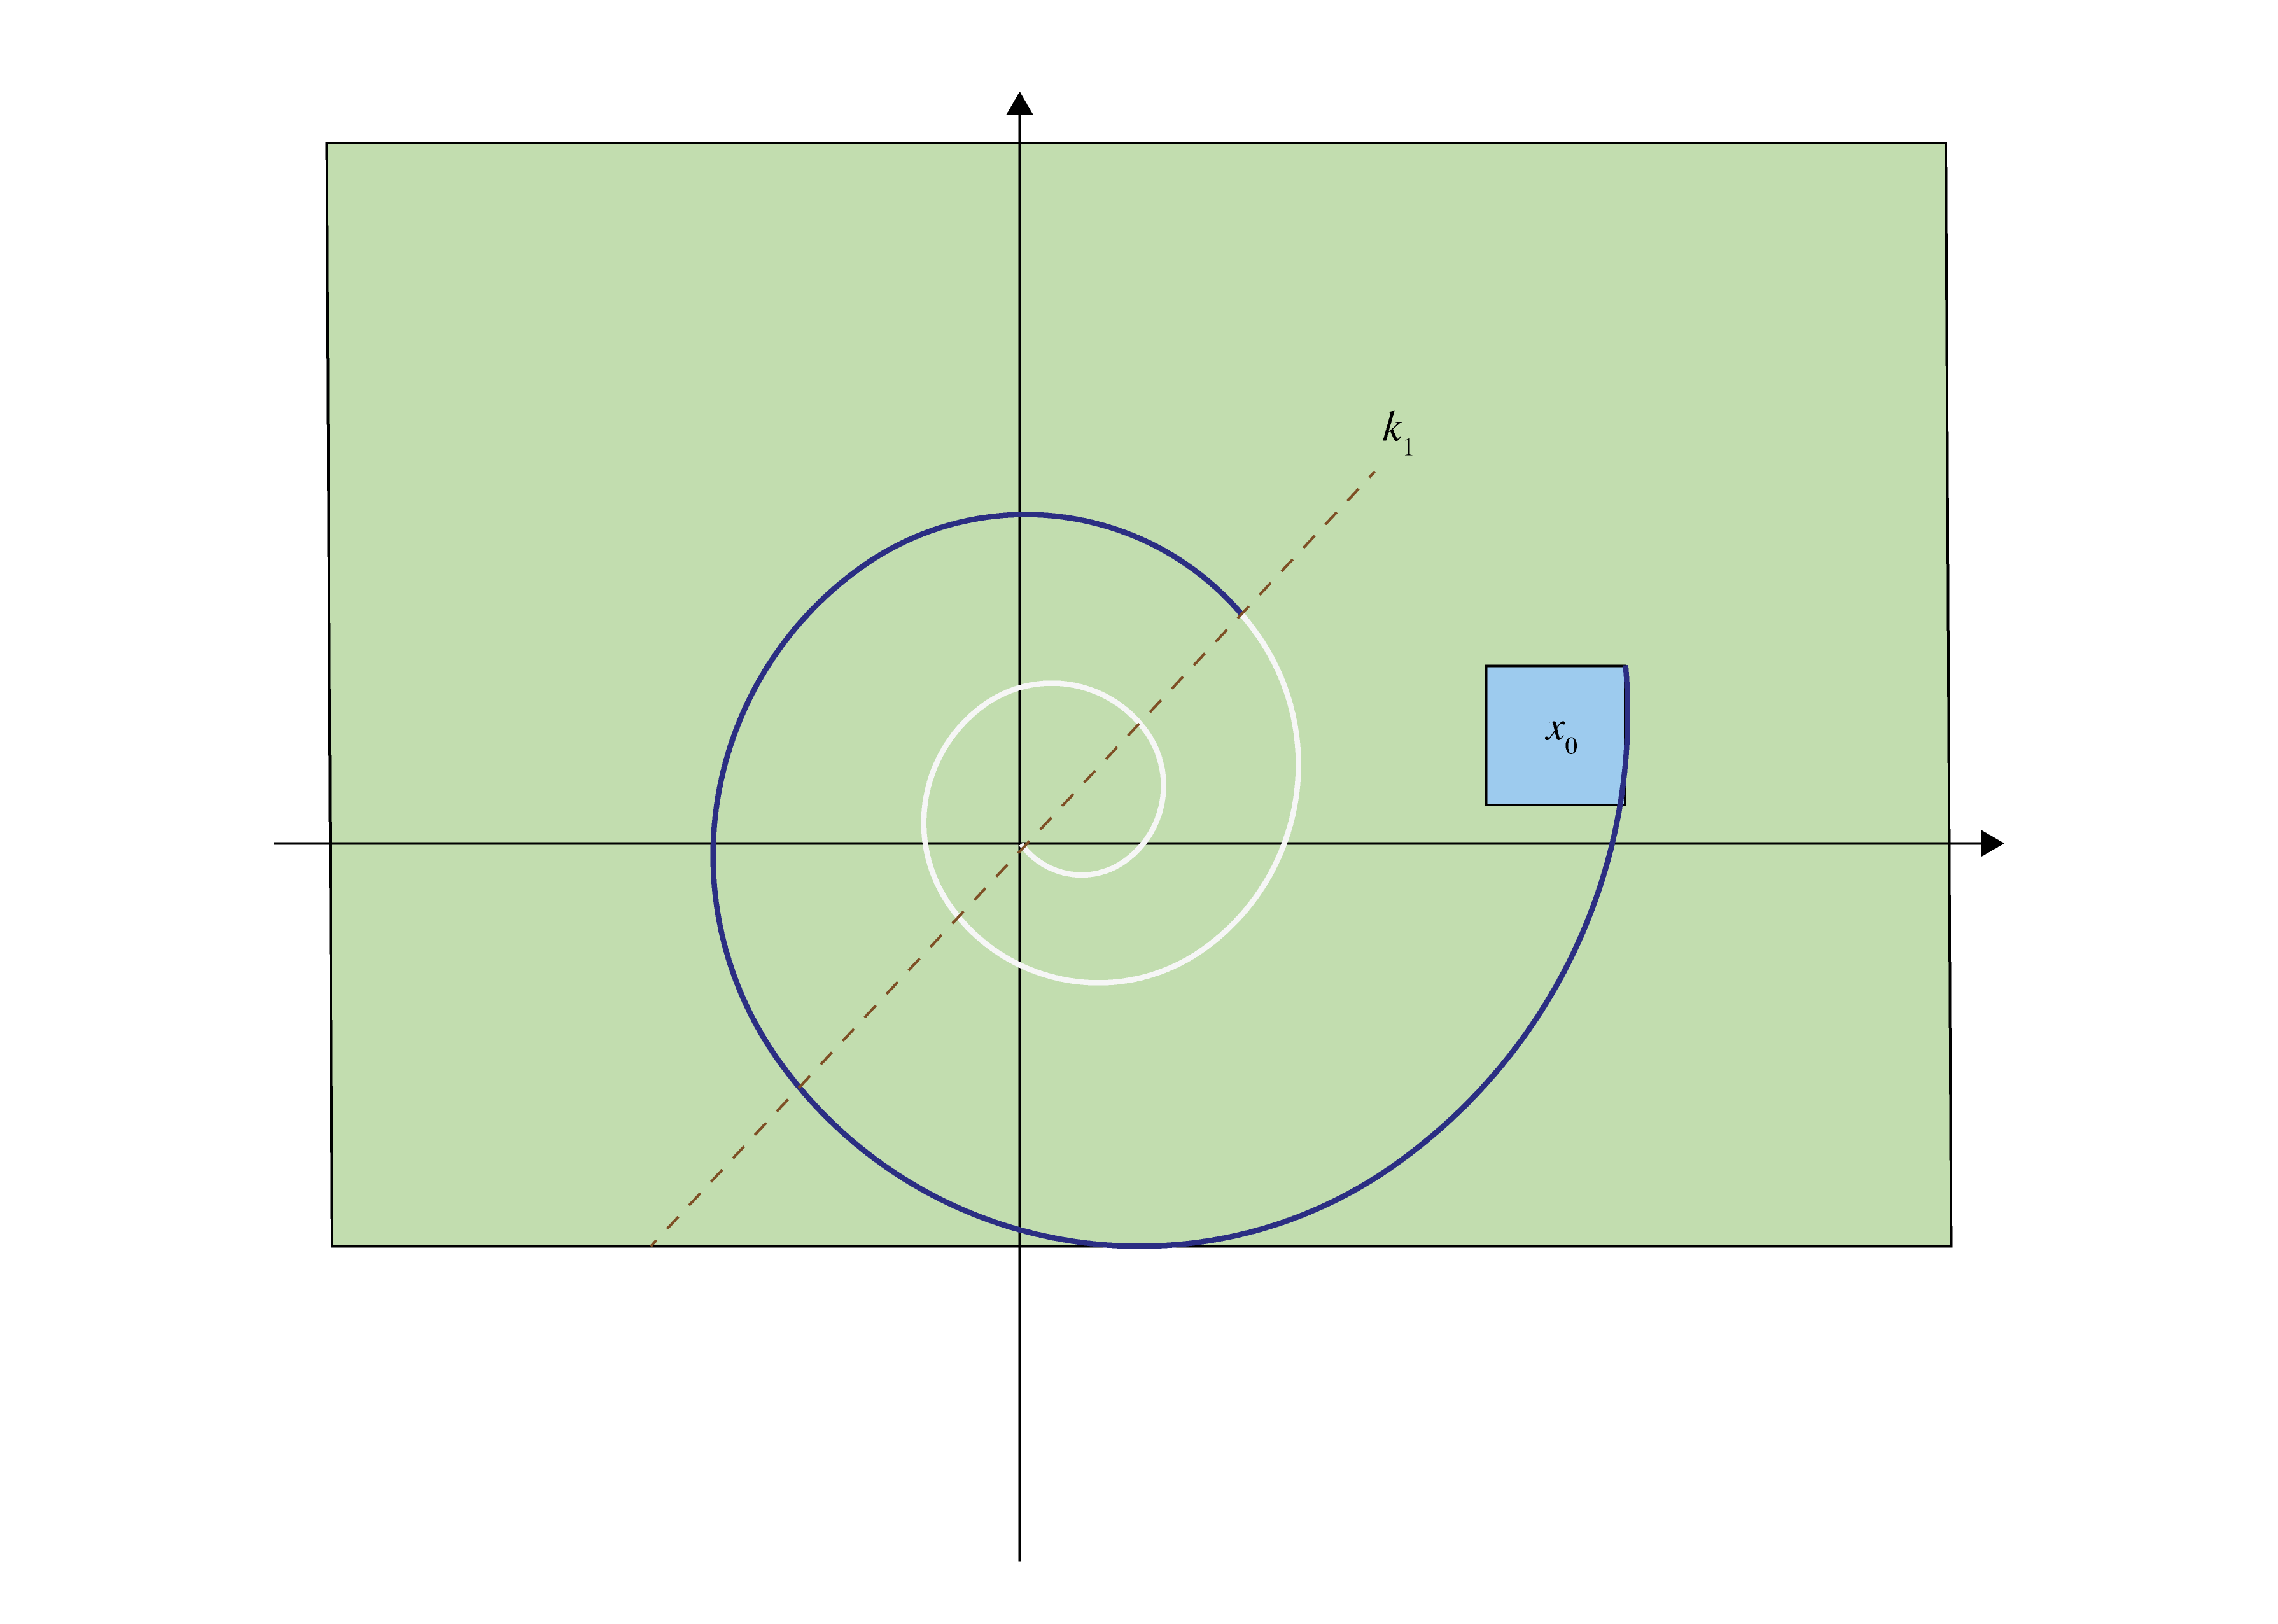
\includegraphics[width=.6\textwidth]{figures/spirals/Spirals-11.png}}
 \only<3>{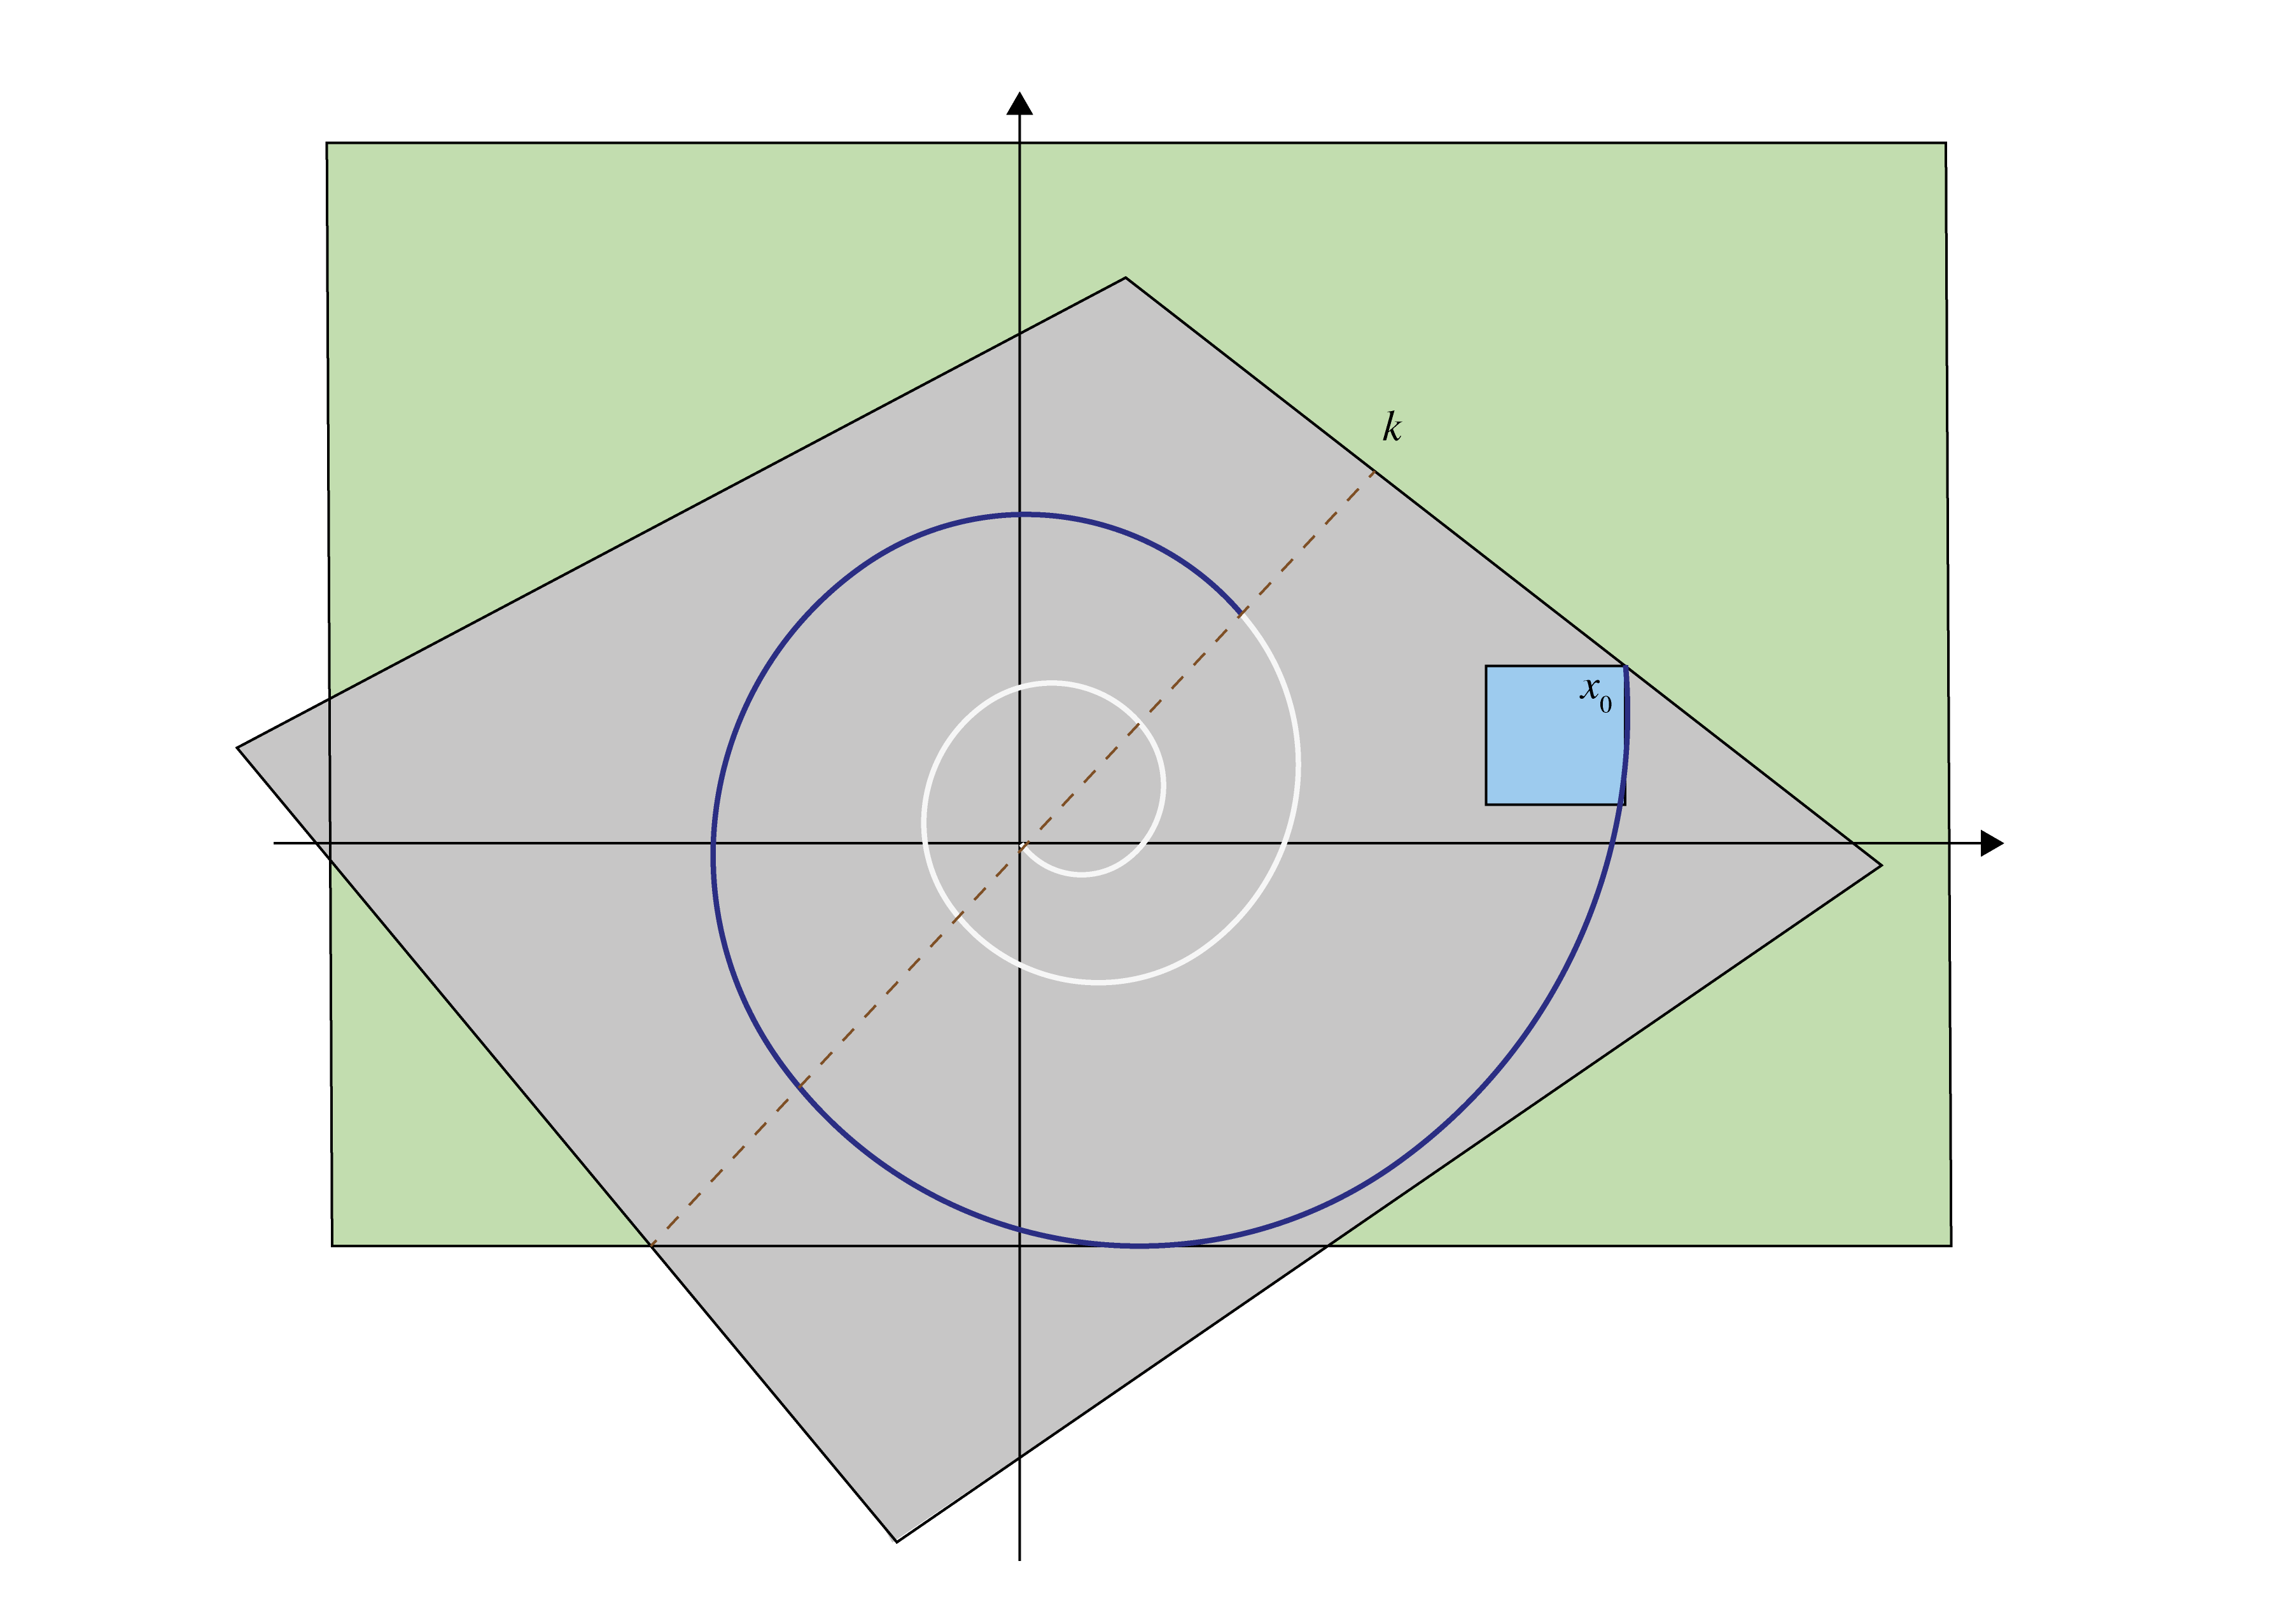
\includegraphics[width=.6\textwidth]{figures/spirals/Spirals-07.png}}
 \only<4>{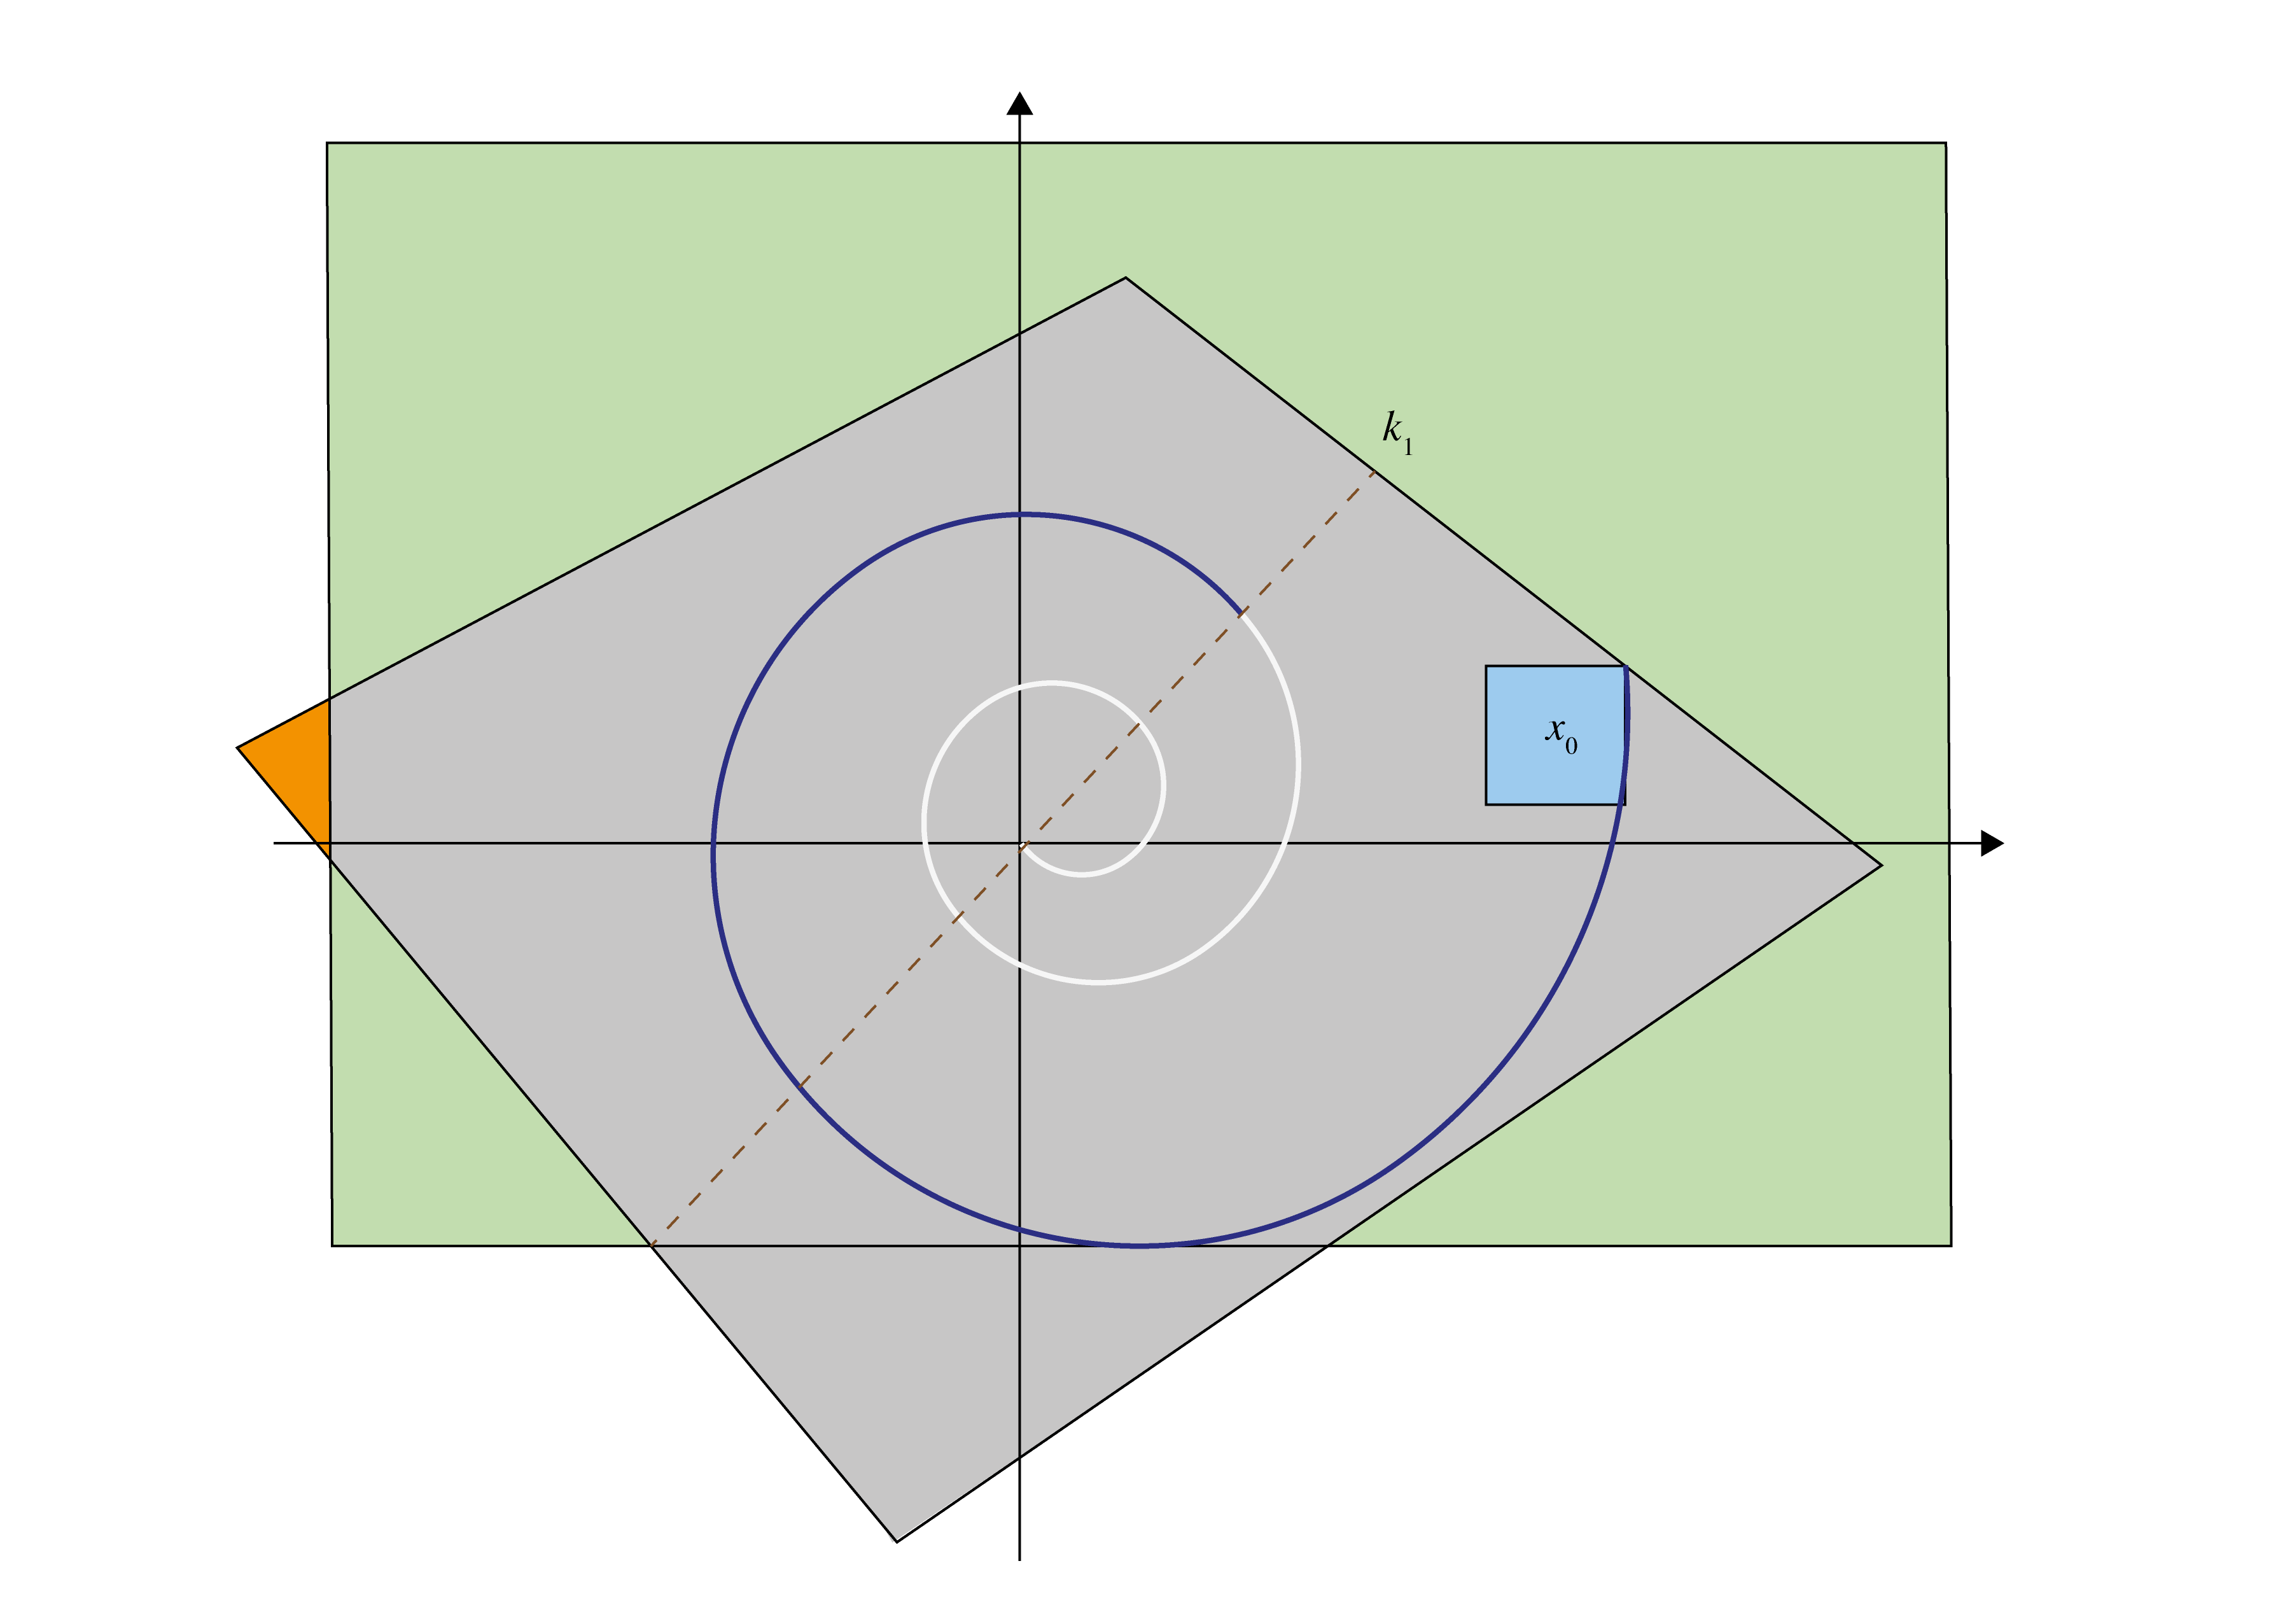
\includegraphics[width=.6\textwidth]{figures/spirals/Spirals-08.png}}
 \only<5>{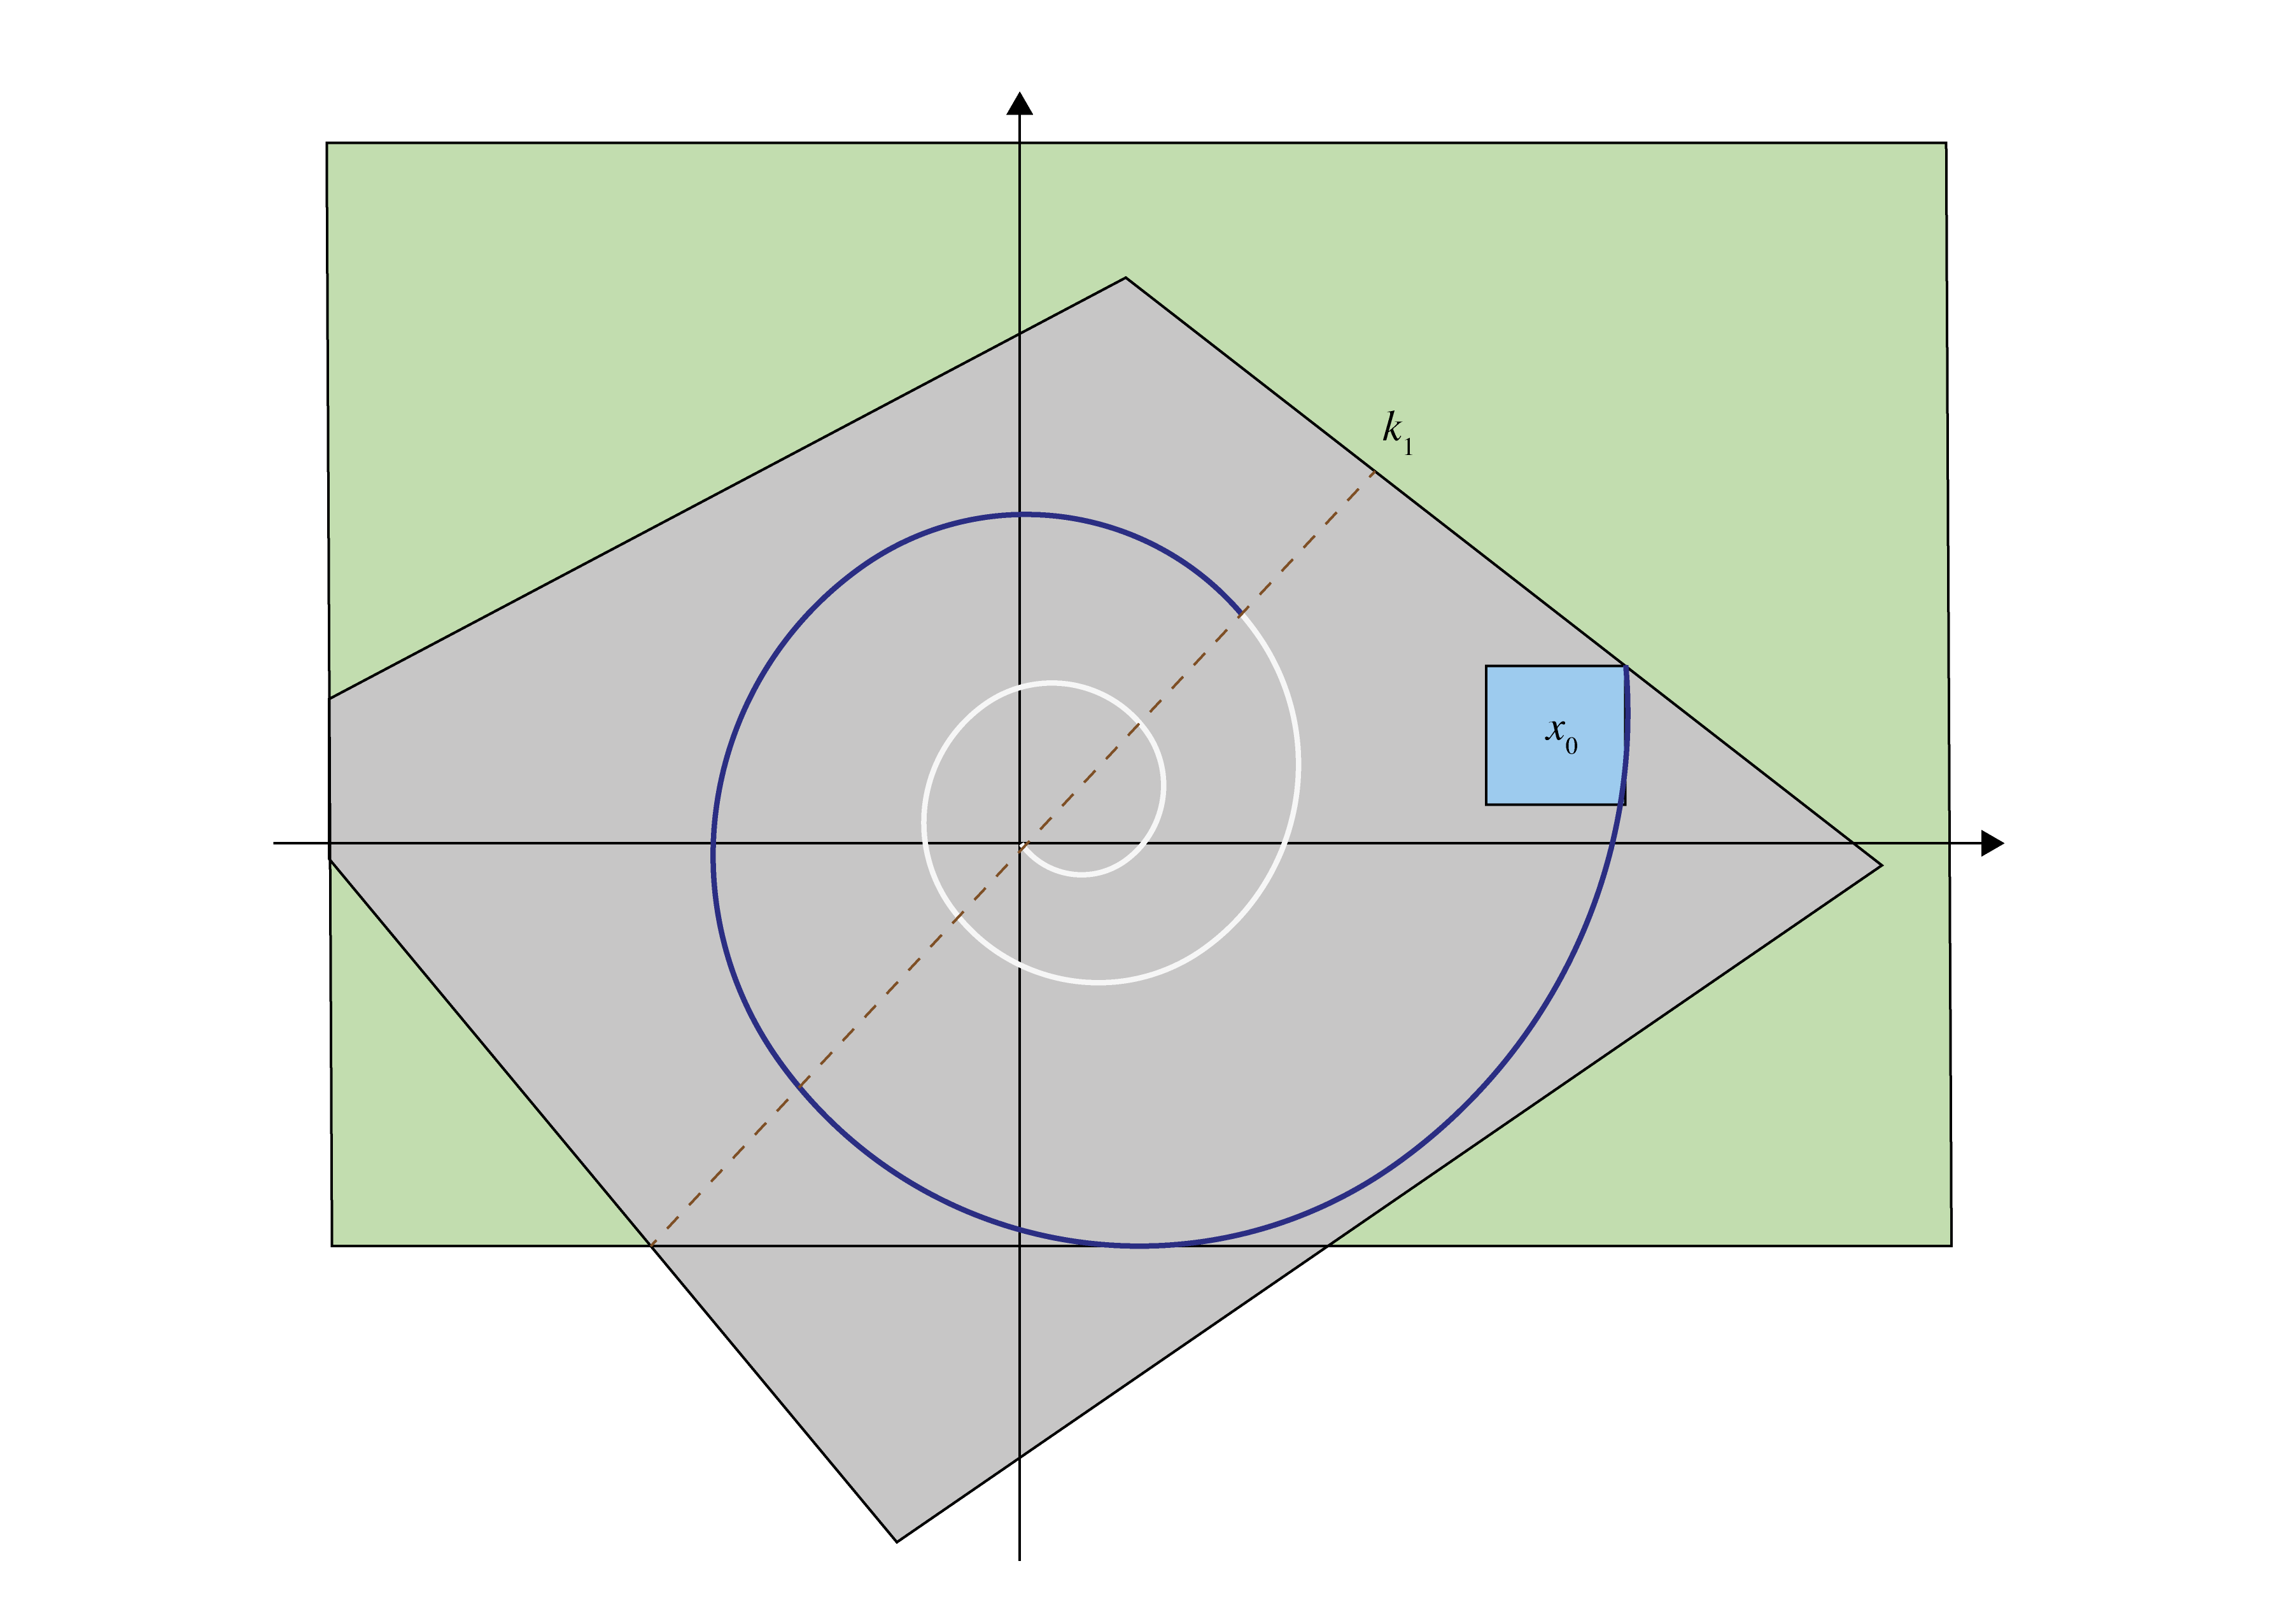
\includegraphics[width=.6\textwidth]{figures/spirals/Spirals-09.png}}    
 \only<6>{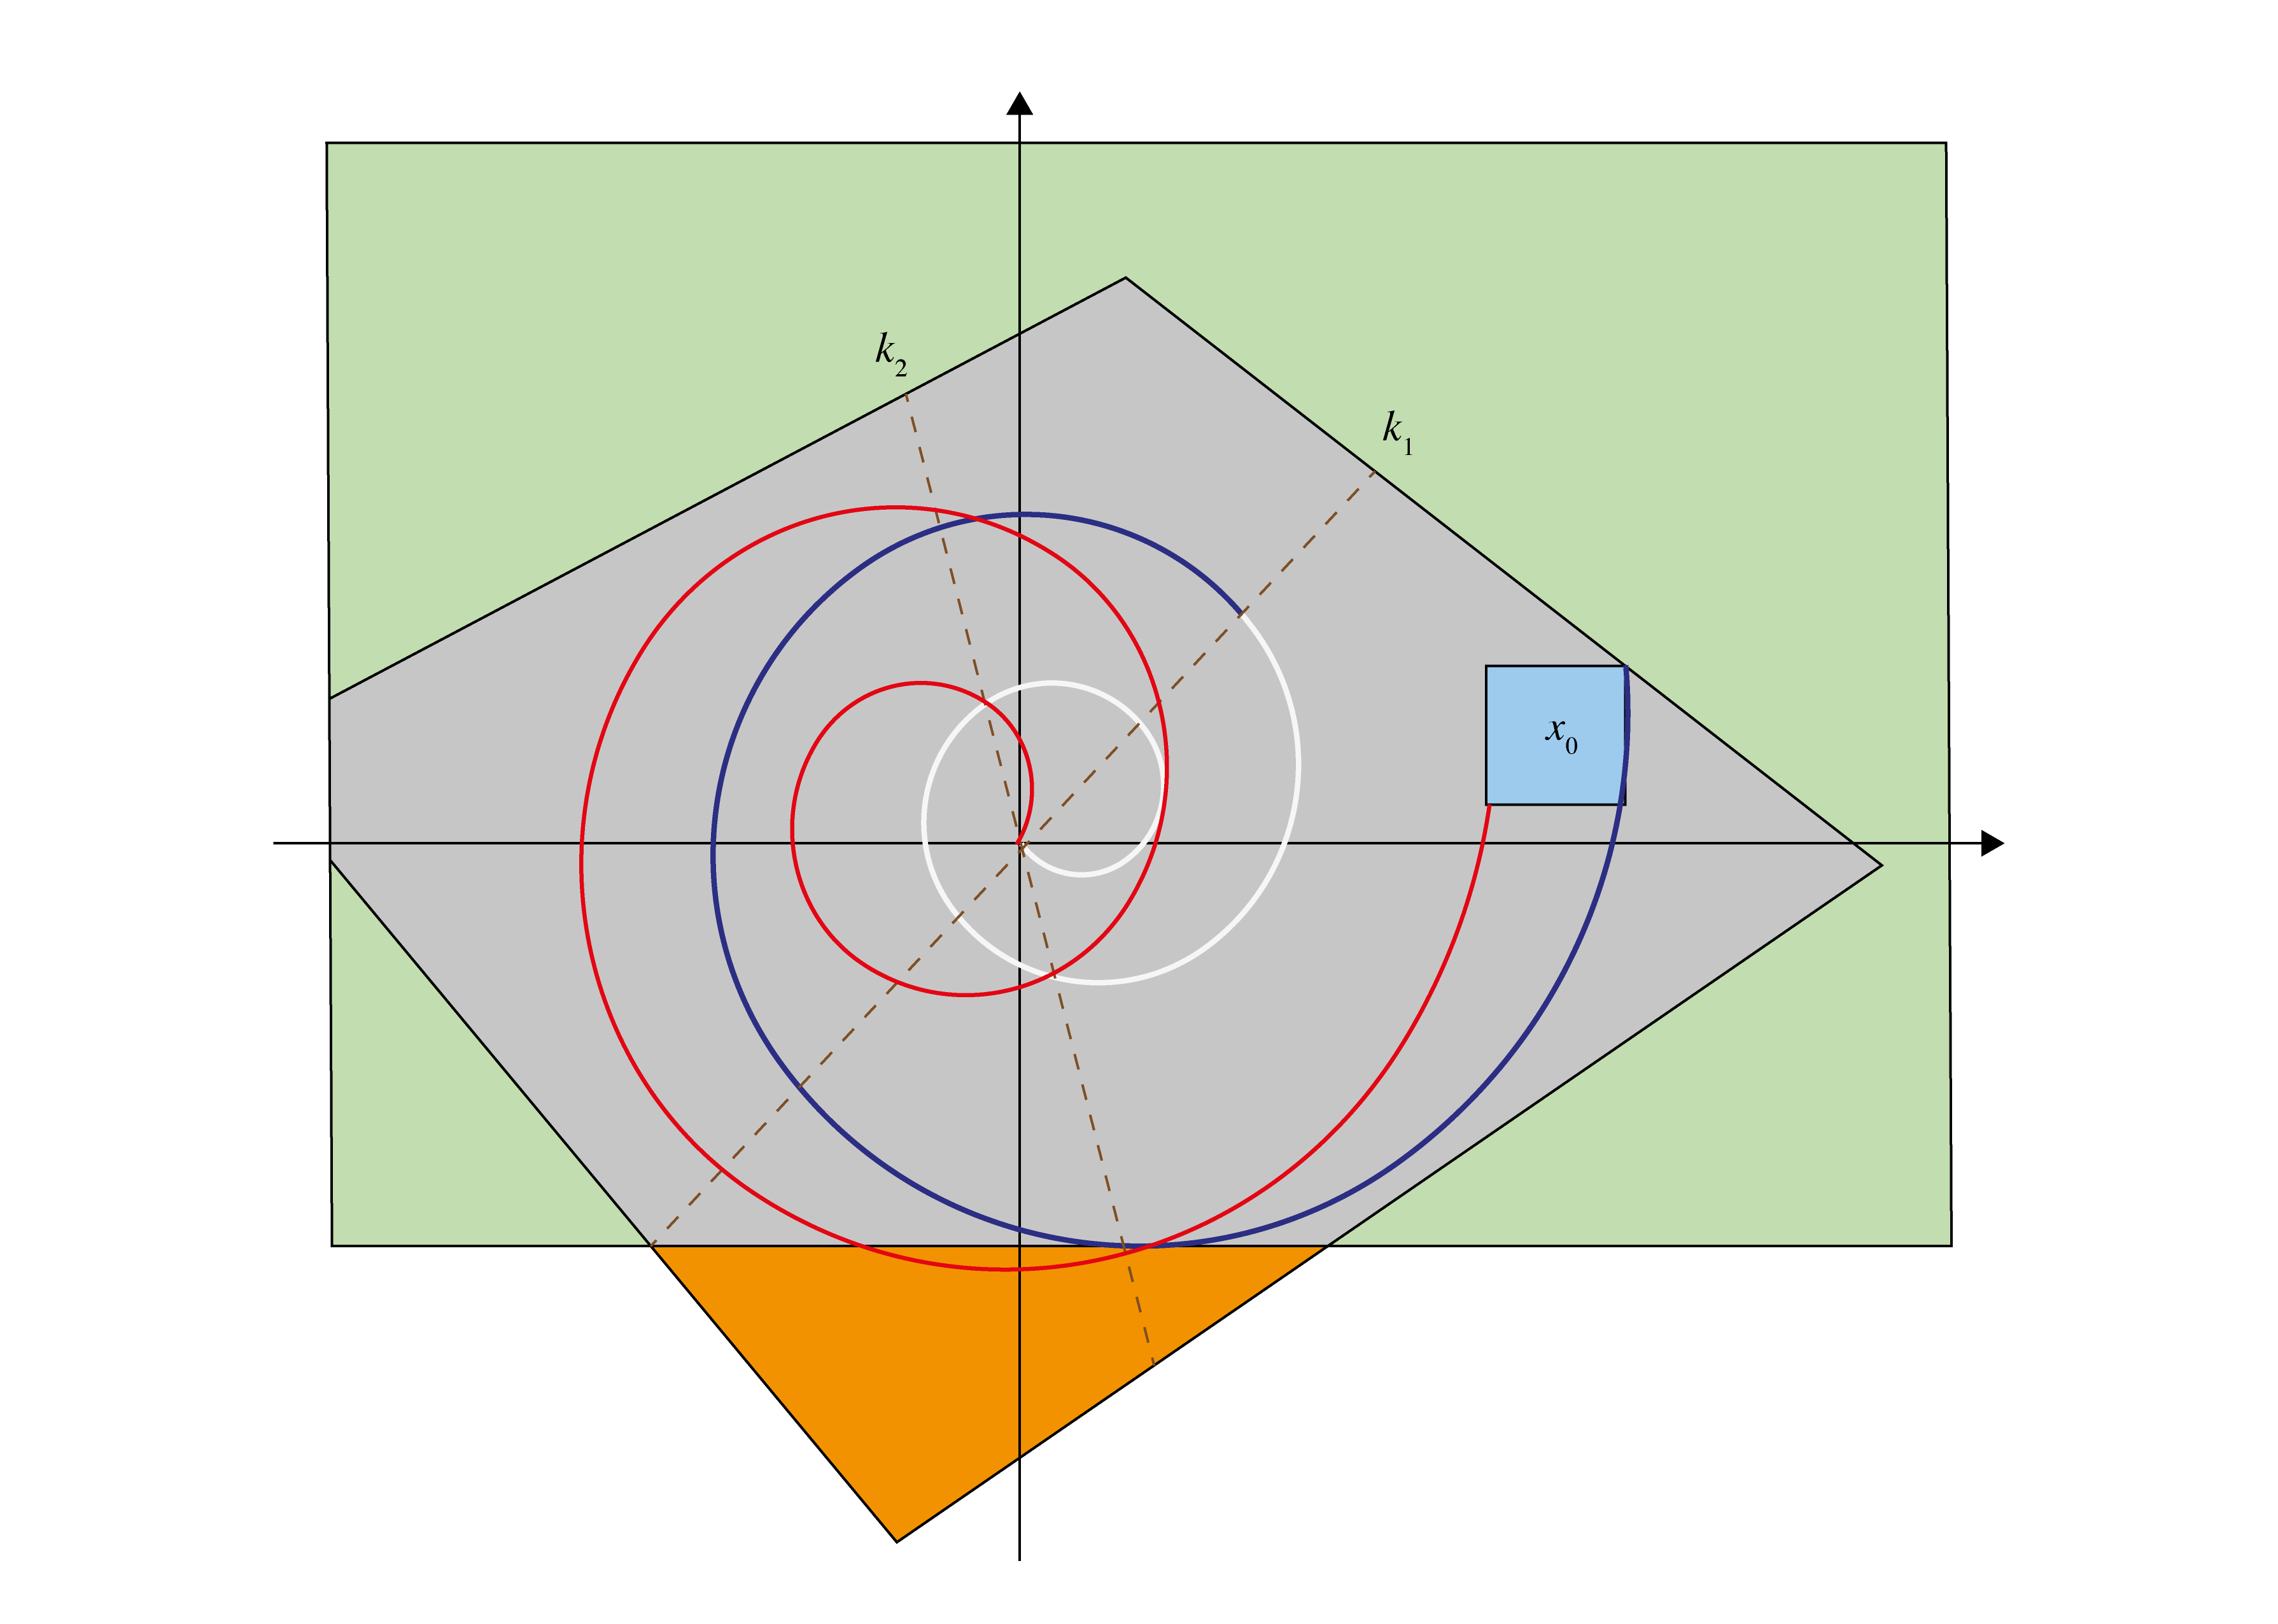
\includegraphics[width=.6\textwidth]{figures/spirals/Spirals-10.png}}
 \only<7>{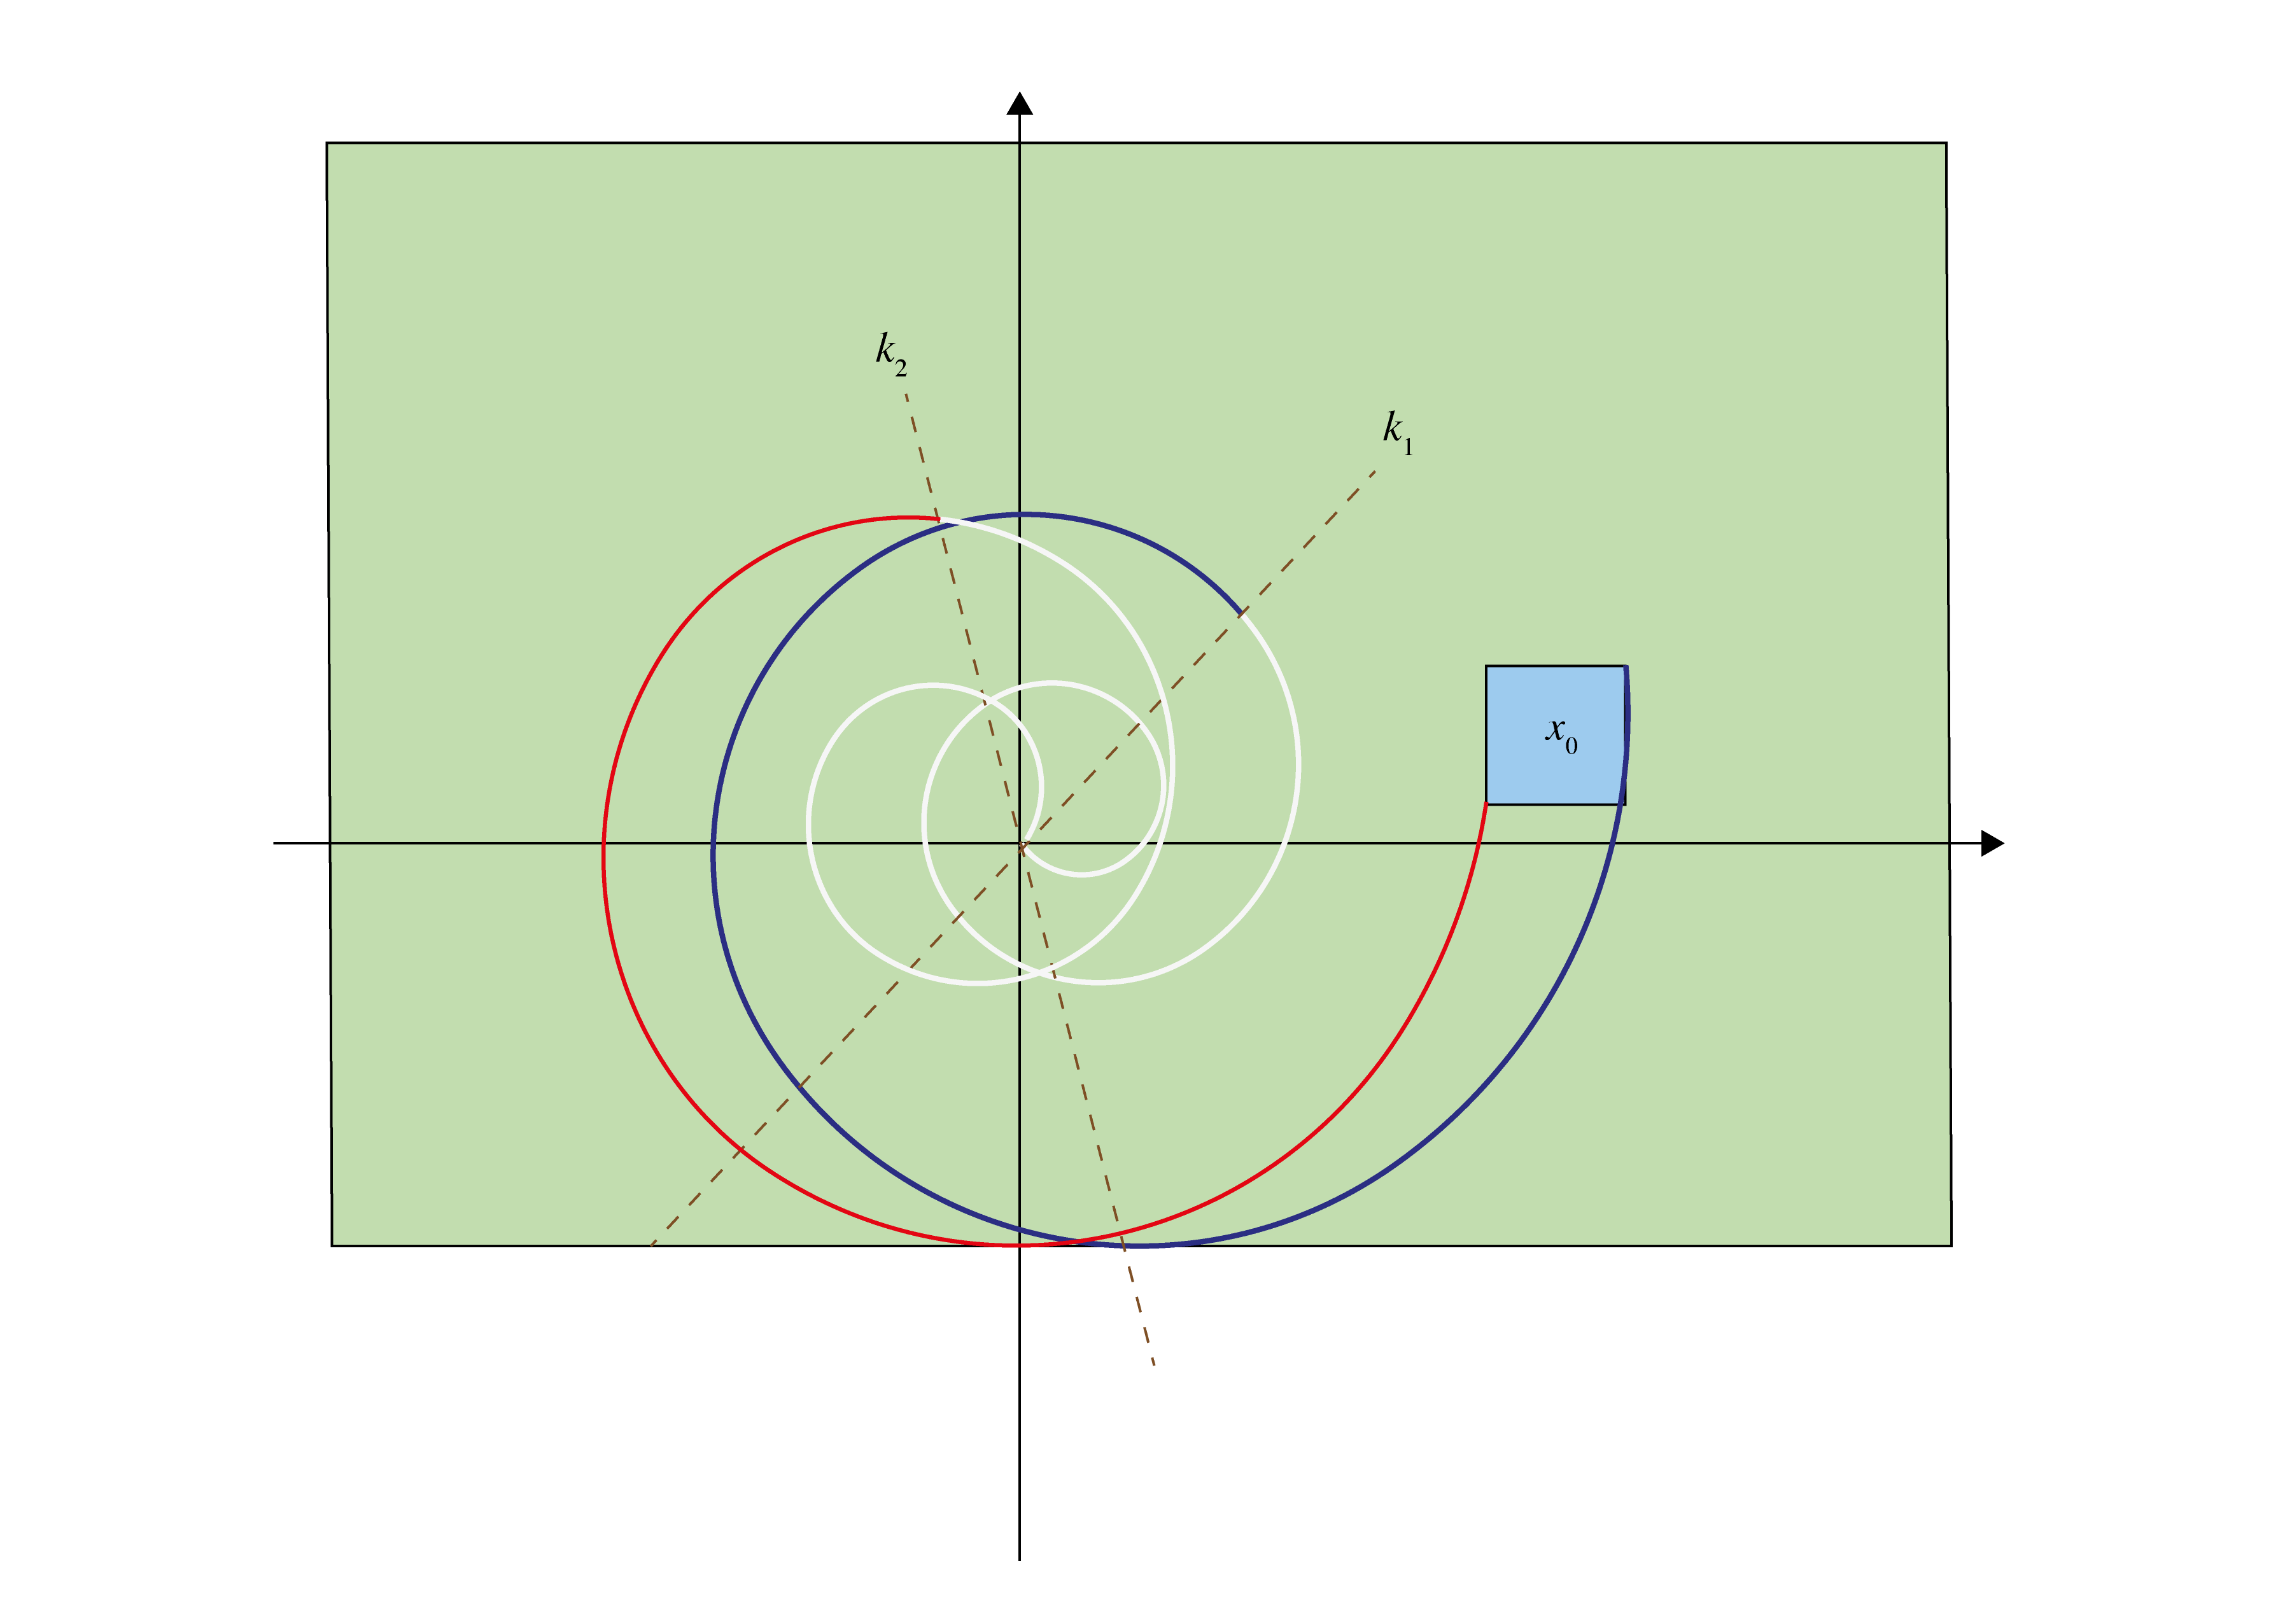
\includegraphics[width=.6\textwidth]{figures/spirals/Spirals-12.png}}
 \only<8->{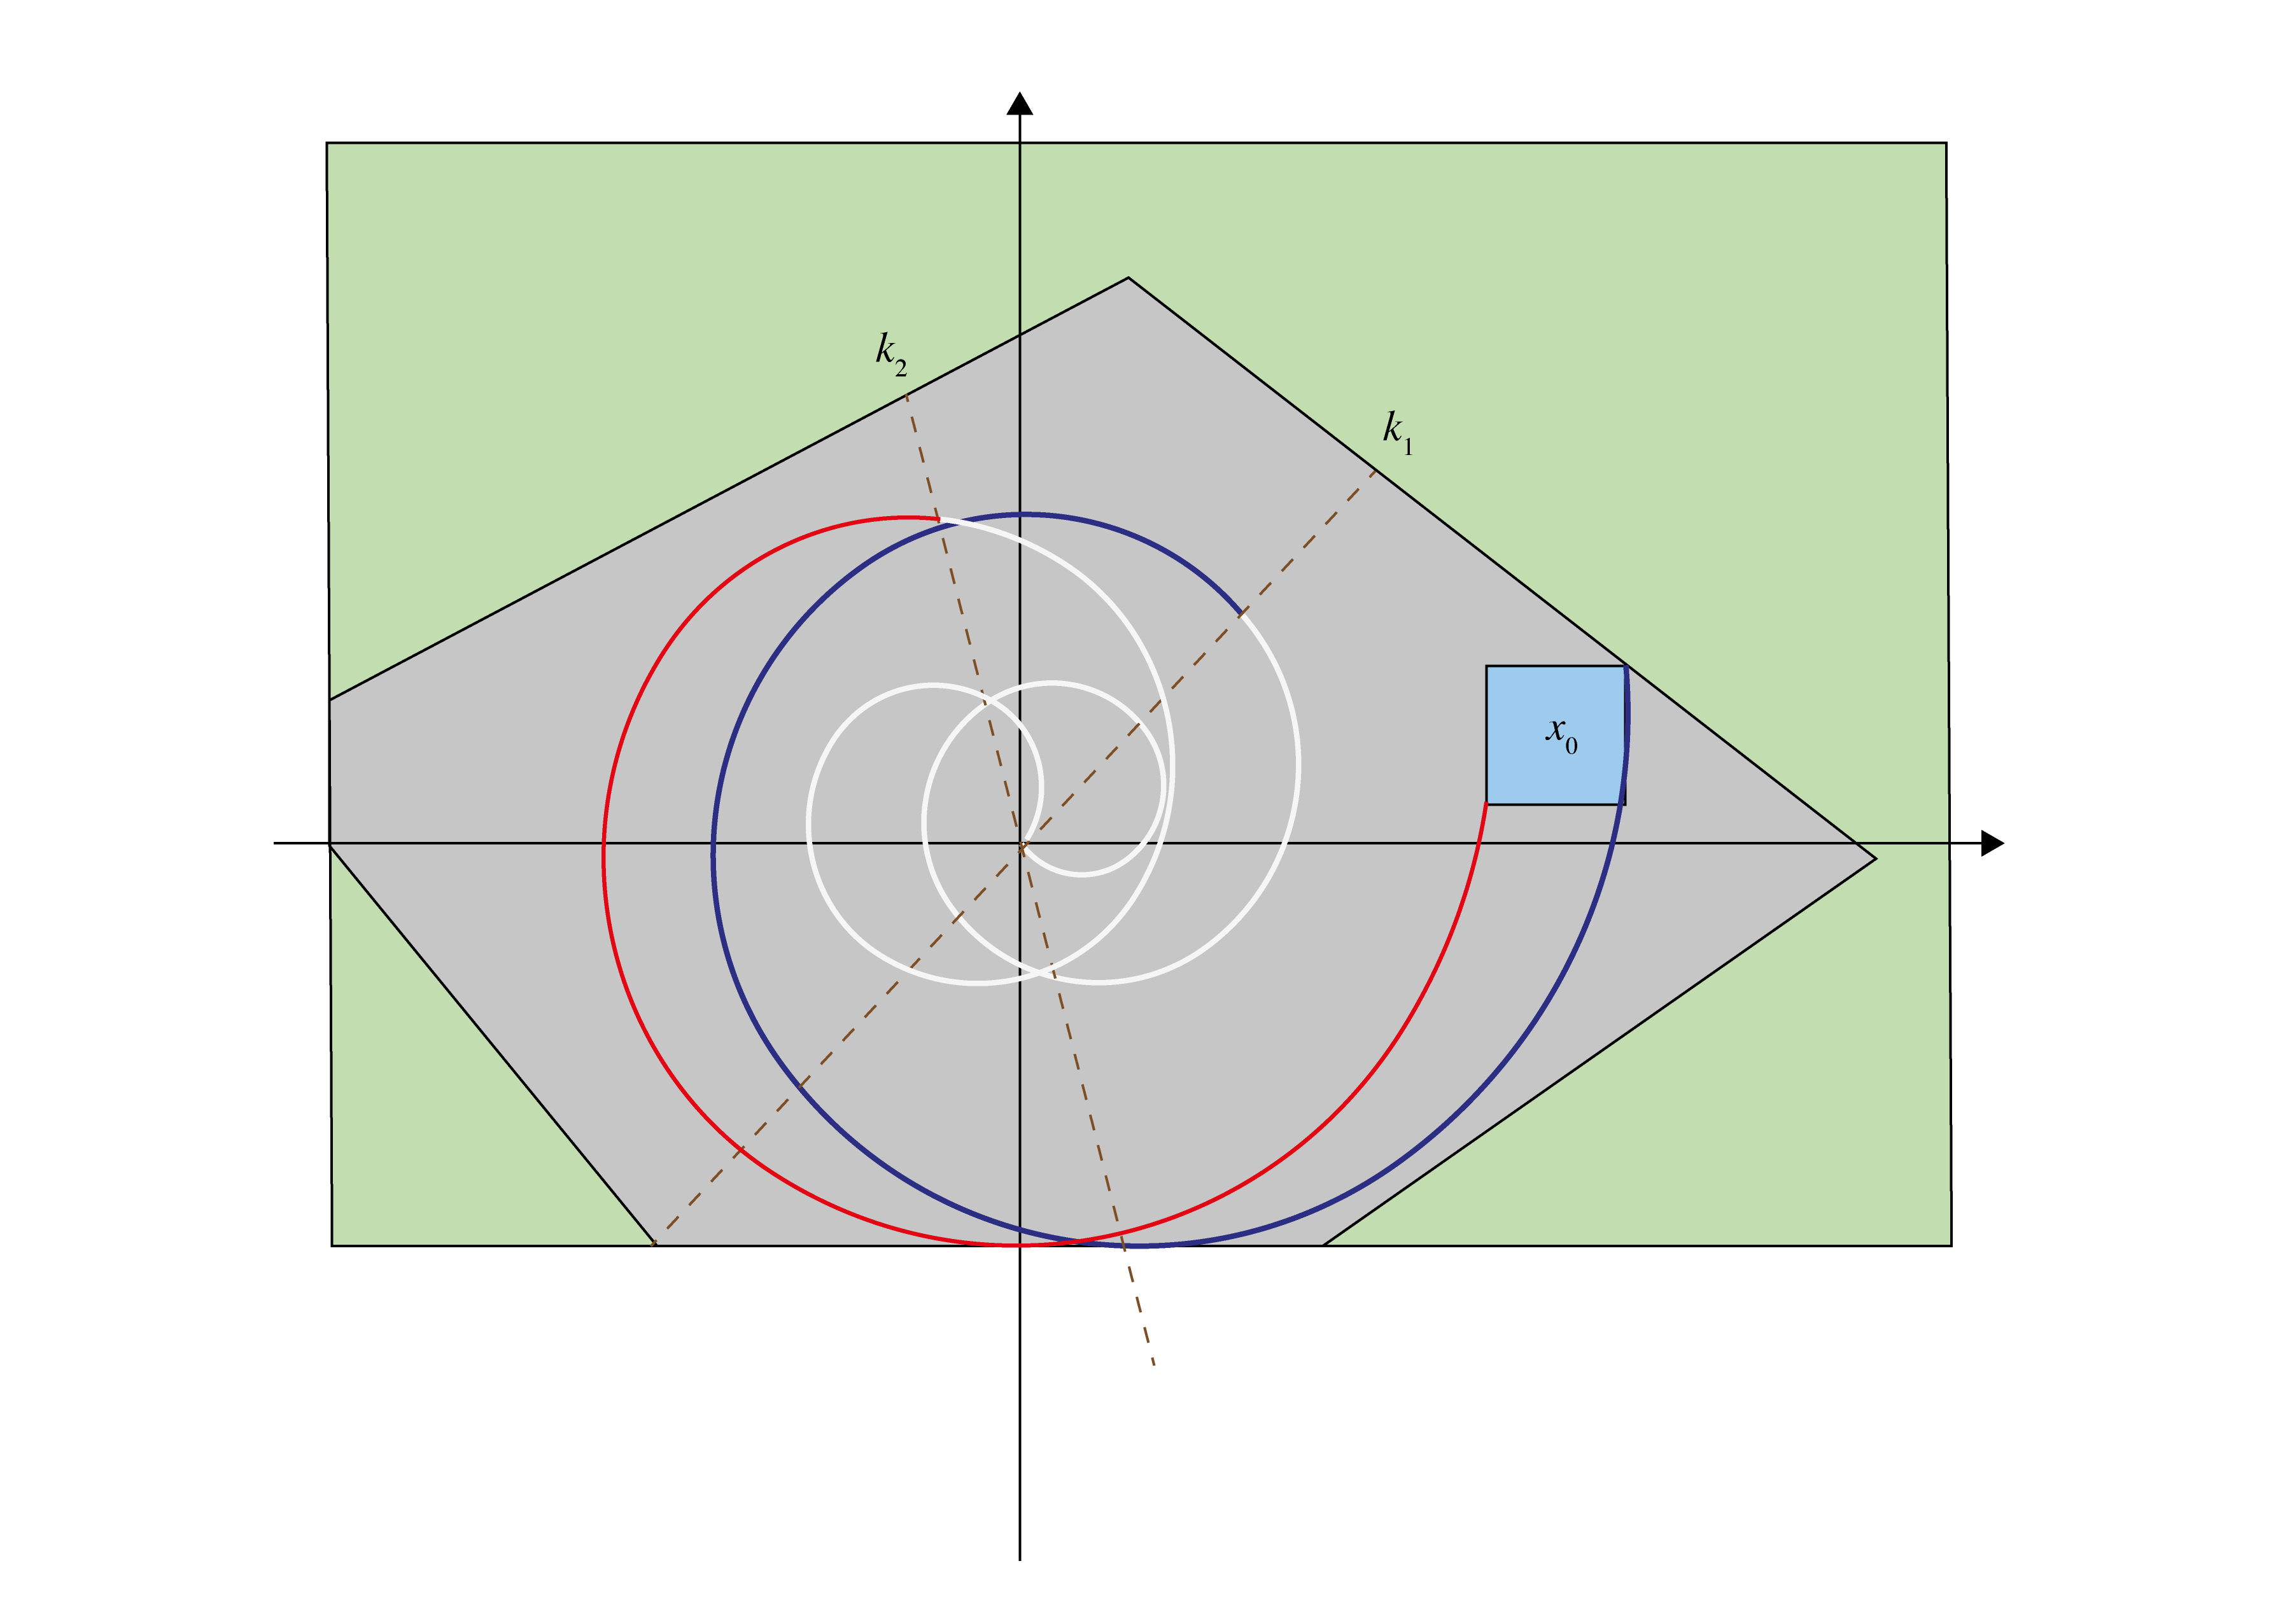
\includegraphics[width=.6\textwidth]{figures/spirals/Spirals-13.png}} 

\end{tabular} 

%[figure]: one spiral with abstract acceleration but no red area, just gray.
 %[figure]: refine abstraction: spiral with two red areas, one spurious and one with a
 % real c-ex.
 %[figure]: two spirals within green area; add grey polygon (inside green area). 
\end{frame}  


\end{document}
